\documentclass[a4paper,12pt]{report}

% ===================================================
% 1. PAGE SETUP & FONTS
% ===================================================
% Margins: Top=3cm, Bottom=3cm, Left=3.5cm, Right=2cm (Standard TCVN)
\usepackage[a4paper,top=3cm,bottom=3cm,left=3.5cm,right=2cm]{geometry}

% Spacing and Indentation
\usepackage{setspace}
\setstretch{1.5} % 1.5 Line spacing
\usepackage{indentfirst} % Indent the first paragraph of every section
\setlength{\parindent}{0.5cm} % Standard 0.5 inch indent (approx 1.27cm)
\setlength{\parskip}{0pt} % Add a little space between paragraphs for readability

% Fonts: Times New Roman setup
\usepackage{iftex}
\ifPDFTeX
  \usepackage[T5]{fontenc}
  \usepackage[utf8]{inputenc}
  \usepackage{mathptmx} % Times New Roman clone for pdfLaTeX
\else
  \usepackage{fontspec}
  \setmainfont{Times New Roman}
\fi

% Fix font size warnings for non-standard sizes
\usepackage{fix-cm}

% Force the "Normal" font size to 13pt (Standard VN requirement)
\makeatletter
\renewcommand\normalsize{%
   \@setfontsize\normalsize{13pt}{16pt}%
   \abovedisplayskip 12\p@ \@plus3\p@ \@minus7\p@
   \abovedisplayshortskip \z@ \@plus3\p@
   \belowdisplayshortskip 6.5\p@ \@plus3.5\p@ \@minus3\p@
   \belowdisplayskip \abovedisplayskip
   \let\@listi\@listI}
\makeatother
\AtBeginDocument{\normalsize}

% ===================================================
% 2. HEADINGS FORMATTING (The Critical Part)
% ===================================================
\usepackage{titlesec}

% --- CHAPTER (Heading 1) ---
% Format: "CHAPTER X: TITLE" - Centered, Bold, Uppercase, 16pt
\titleformat{\chapter}[block]
  {\centering\normalfont\bfseries\fontsize{16}{19}\selectfont\MakeUppercase} % Format
  {\chaptertitlename\ \thechapter:} % Label (e.g., "CHAPTER 1:")
  {0.5em} % Space between label and title
  {} % Before code

% Adjust spacing around Chapter titles
\titlespacing*{\chapter}{0pt}{-10pt}{20pt} 
% {Left}{Before (negative pulls it up)}{After}

% --- SECTION (Heading 2) ---
% Format: "1.1 Title" - Left, Bold, 13pt
\titleformat{\section}
  {\normalfont\bfseries\fontsize{13}{16}\selectfont}
  {\thesection}{1em}{}
\titlespacing*{\section}{0pt}{12pt}{6pt}

% --- SUBSECTION (Heading 3) ---
% Format: "1.1.1 Title" - Left, Bold, 13pt
\titleformat{\subsection}
  {\normalfont\bfseries\fontsize{13}{16}\selectfont}
  {\thesubsection}{1em}{}
\titlespacing*{\subsection}{0pt}{12pt}{6pt}

% --- SUBSUBSECTION (Heading 4) ---
% Format: "1.1.1.1 Title" - Left, Italic, 13pt
\titleformat{\subsubsection}
  {\normalfont\itshape\fontsize{13}{16}\selectfont}
  {\thesubsubsection}{1em}{}
\titlespacing*{\subsubsection}{0pt}{12pt}{6pt}

% Numbering depth
\setcounter{secnumdepth}{4}
\setcounter{tocdepth}{3}

% ===================================================
% 3. CAPTIONS & REFERENCES
% ===================================================
\usepackage{graphicx}
\usepackage{tikz}
\usetikzlibrary{calc}
\usepackage{caption}
\usepackage{float} % provides the [H] placement option
\usepackage{xurl} % allow URL line breaks to fix overfull \hbox
\usepackage[hidelinks]{hyperref}
\usepackage{listings}
\usepackage{xcolor}

% Define colors for code listings
\definecolor{codegray}{rgb}{0.9,0.9,0.9}
\lstset{
    backgroundcolor=\color{codegray},
    basicstyle=\ttfamily\small,
    breaklines=true,
    frame=single,
    rulecolor=\color{lightgray},
    showstringspaces=false
}

% Caption styling: Label Bold, Text Italic
\captionsetup{labelfont=bf,textfont=it,labelsep=colon}

% --- LANGUAGE SETTINGS ---
% UNCOMMENT the pair you need:

% OPTION A: ENGLISH (Standard)
% \renewcommand{\chaptername}{CHAPTER}
% \renewcommand{\figurename}{Figure}
% \renewcommand{\tablename}{Table}
% \renewcommand{\contentsname}{TABLE OF CONTENTS}

% OPTION B: VIETNAMESE (Standard)
\renewcommand{\chaptername}{CHƯƠNG}
\renewcommand{\figurename}{Hình}
\renewcommand{\tablename}{Bảng}
\renewcommand{\contentsname}{MỤC LỤC}
\renewcommand{\listfigurename}{DANH MỤC HÌNH ẢNH}

% ===================================================
% 4. HEADER & FOOTER
% ===================================================
\usepackage{fancyhdr}
\pagestyle{fancy}
\fancyhf{}
\fancyfoot[C]{\thepage} % Page number bottom center
\renewcommand{\headrulewidth}{0pt} % No line at top
\renewcommand{\footrulewidth}{0pt}

% ===================================================
% DOCUMENT BEGINS
% ===================================================
\begin{document}

% --- TITLE PAGE ---
\begin{titlepage}
\begin{tikzpicture}[remember picture, overlay]
    \draw[line width = 4.5pt] ($(current page.north west) + (3.0cm,-2.0cm)$) rectangle ($(current page.south east) + (-2.0cm,2.0cm)$);
\end{tikzpicture}

\centering
\vspace*{0.5cm}
{\fontsize{13}{15}\selectfont \textbf{ĐẠI HỌC CẦN THƠ}\par}
{\fontsize{13}{15}\selectfont \textbf{TRƯỜNG CÔNG NGHỆ THÔNG TIN \& TRUYỀN THÔNG}\par}

\vspace{0.5cm}
\begin{figure}[h]
    \centering
    
\includegraphics[width=3cm]{./assets/logo-ctu.png}
\end{figure}
\vspace{0.5cm}

{\fontsize{18}{22}\selectfont \textbf{BÁO CÁO}\par}
{\fontsize{18}{22}\selectfont \textbf{PHÁT TRIỂN ỨNG DỤNG WEB}\par}
{\fontsize{18}{22}\selectfont \textbf{CT449}\par}

\vspace{1cm}

{\fontsize{13}{15}\selectfont \textbf{Bài Tập}\par}
{\fontsize{20}{24}\selectfont \textbf{BACKEND}\par}

\vspace{2cm}

\begin{flushleft}
\hspace{2cm}
\begin{tabular}{ll}
\textbf{Giảng viên hướng dẫn:} & Ths. Nguyễn Minh Trung \\
\textbf{Sinh viên thực hiện:} & Trần Thanh Duy \\
\textbf{MSSV:} & DC24V7X604 \\
\end{tabular}
\end{flushleft}

\vfill
{\fontsize{13}{15}\selectfont \textbf{Cần Thơ, năm 2026}\par}
\end{titlepage}

% --- FRONT MATTER ---
\pagenumbering{roman} % i, ii, iii...

\phantomsection
\addcontentsline{toc}{chapter}{\contentsname}
\tableofcontents
\clearpage

\phantomsection
\addcontentsline{toc}{chapter}{\listfigurename}
\listoffigures
\clearpage

% --- MAIN CONTENT ---
\pagenumbering{arabic} % 1, 2, 3...
\setcounter{page}{1}

% CHAPTER 1
\chapter{BACKEND 1} % Will automatically print "CHAPTER 1: INTRODUCTION"
\section{Cài đặt môi trường node và git}
Thực hiện tải nodejs và git theo hướng dẫn.

Sau đó kiểm tra bằng lệnh như ảnh:

\begin{figure}[H]
    \centering
    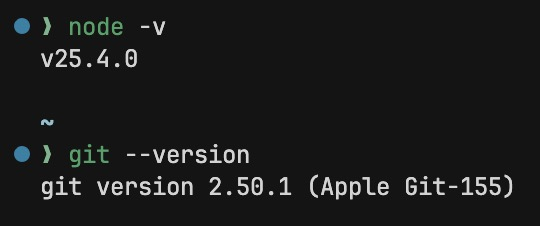
\includegraphics[width=0.8\textwidth]{./assets/img1.jpg}
    \caption{Kiểm tra môi trường}
    \label{fig:check_env}
\end{figure}

\section{Tạo thư mục Node}

Thực hiện npm init


\begin{figure}[H] % ht to H put it here or nowhere else to prevent floating
    \centering
    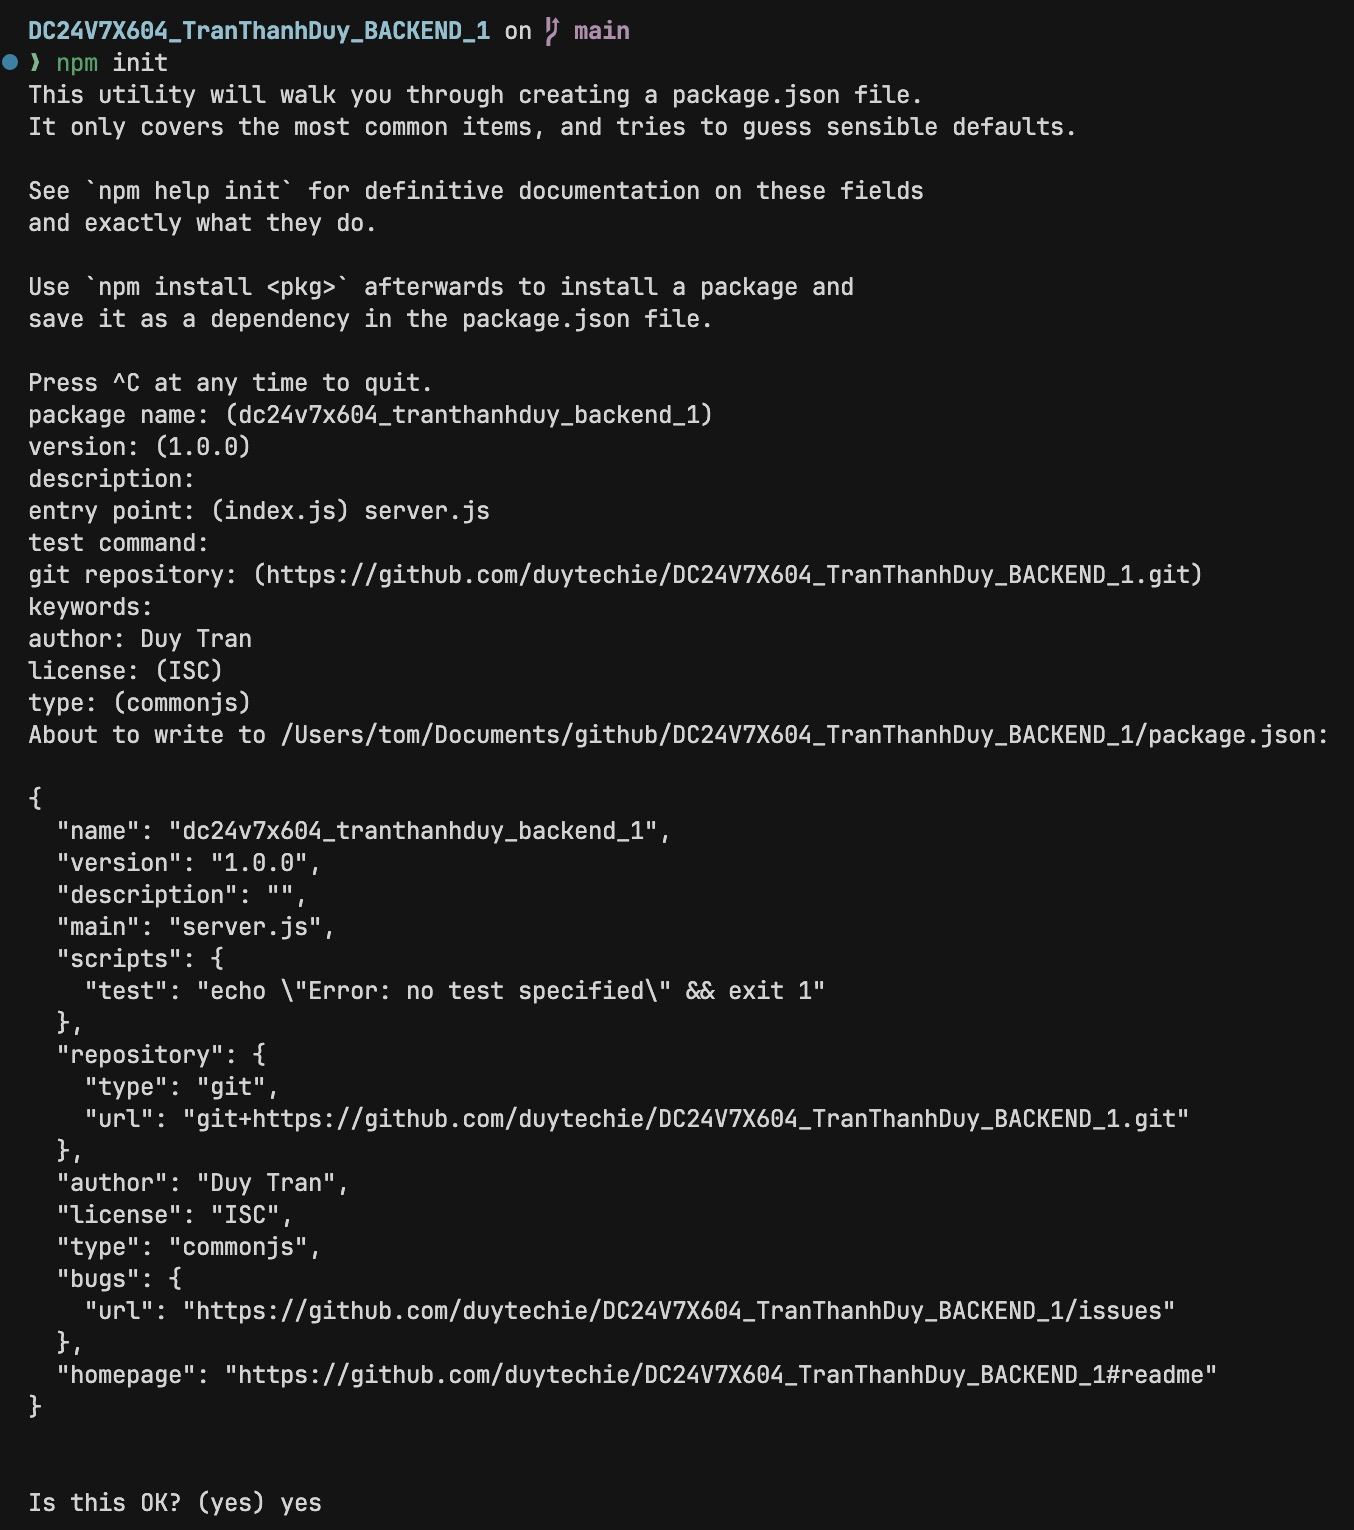
\includegraphics[width=0.8\textwidth]{./assets/img2.jpg}
    \caption{npm init}
    \label{fig:npm_init}
\end{figure}

Cài package cần thiết:

\begin{figure}[H]
    \centering
    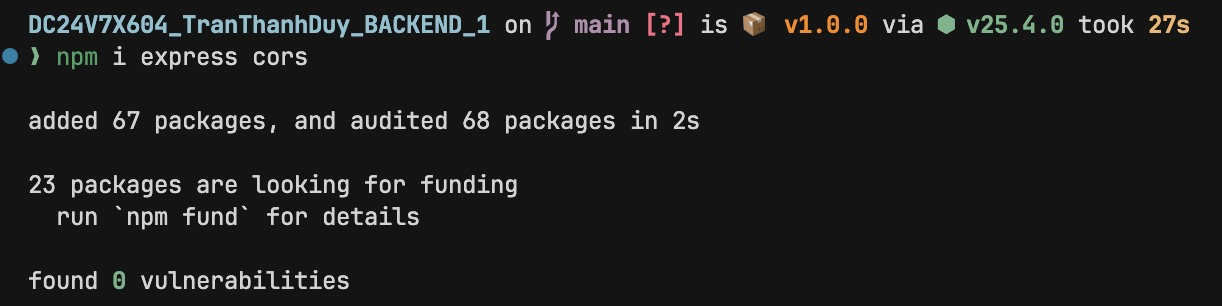
\includegraphics[width=0.8\textwidth]{./assets/img3.jpg}
    \caption{Cài package cần thiết}
    \label{fig:install_pkg}
\end{figure}

% \section{Objectives}
% Here is a citation example.

\section{Quản lý dự án bởi Git và Github}

Tạo file \texttt{.gitignore} để loại trừ thư mục \texttt{node\_modules} chứa các thư viện Node.js.

Lần lượt thực hiện các lệnh của Git để đẩy code lên Github:
\begin{itemize}
    \item \texttt{git init}~-- Khởi tạo kho lưu trữ Git mới.
    \item \texttt{git add -A} Thêm tất cả các tệp hiện tại vào vùng staging.
    \item \texttt{git commit -m ""}~-- Tạo commit đầu tiên với lời nhắn.
    \item \texttt{git push origin main}~-- Đẩy code lên Github.
\end{itemize}

\begin{figure}[H]
    \centering
    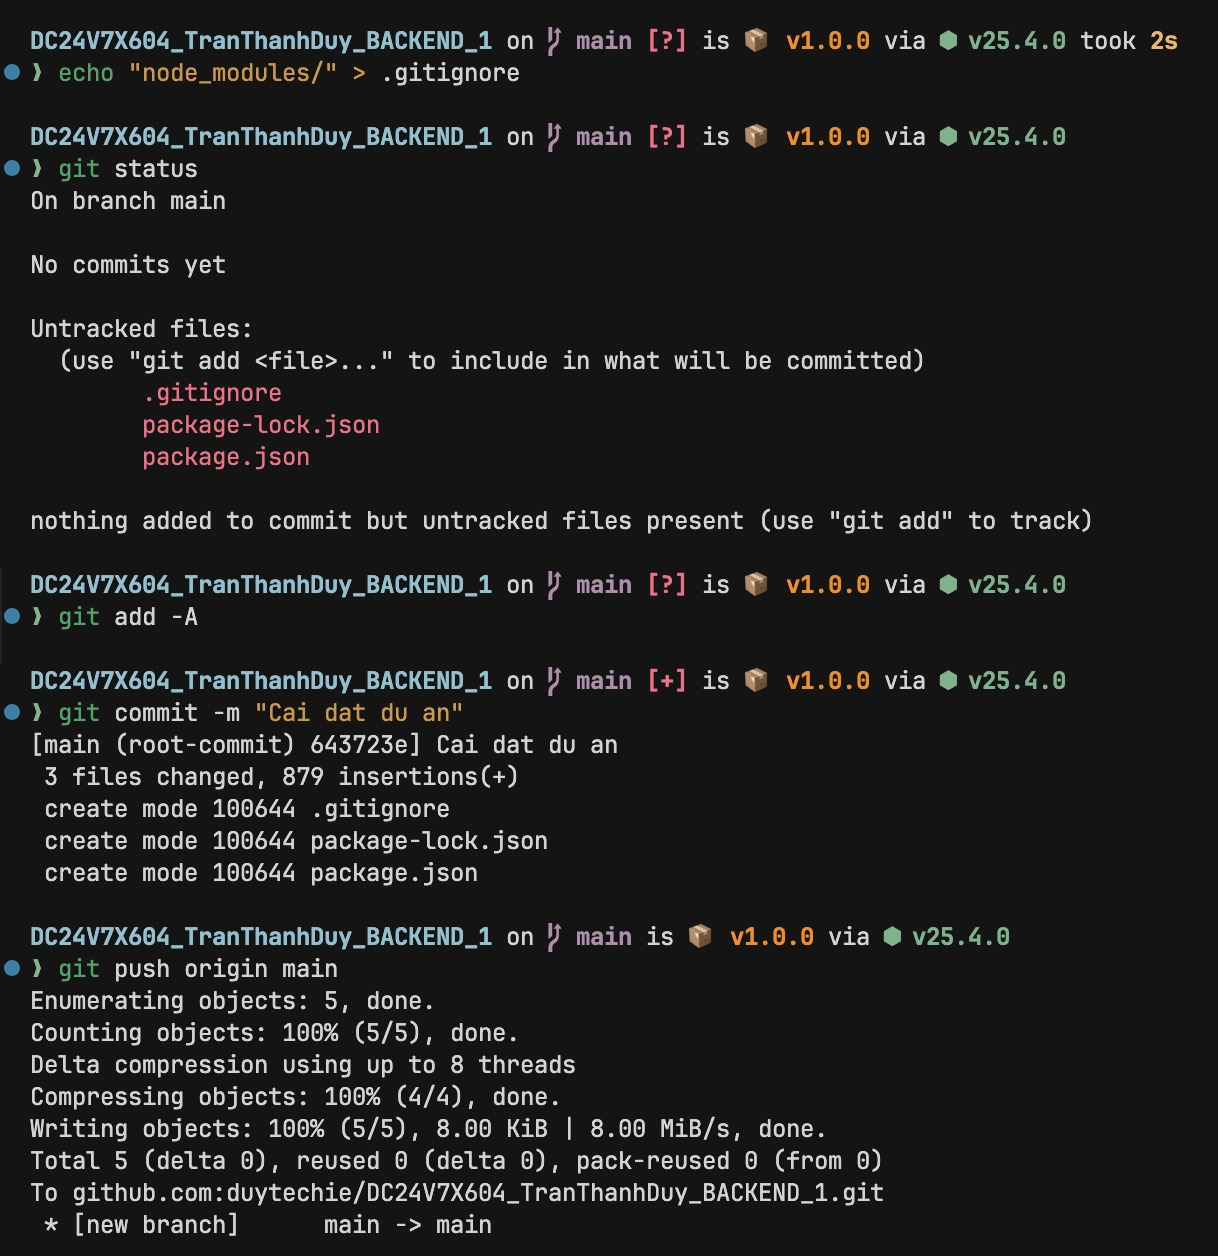
\includegraphics[width=0.8\textwidth]{./assets/img8.jpg}
    \caption{Cài package cần thiết}
    \label{fig:git}
\end{figure}

\section{Cấu hình Visual Studio Code, Eslint, Prettier}

Cài đặt extension Prettier và ESLint trên Visual Studio Code (Cursor).

\begin{figure}[H]
  \centering
  
\includegraphics[width=0.8\textwidth]{./assets/img9.jpg}
  \caption{Extension Prettier và ESLint}
  \label{fig:vscode_extension1}
\end{figure}

Kích hoạt tính năng \texttt{formatOnPaste} và \texttt{formatOnSave} trên \texttt{settings.json}.

\begin{figure}[H]
  \centering
  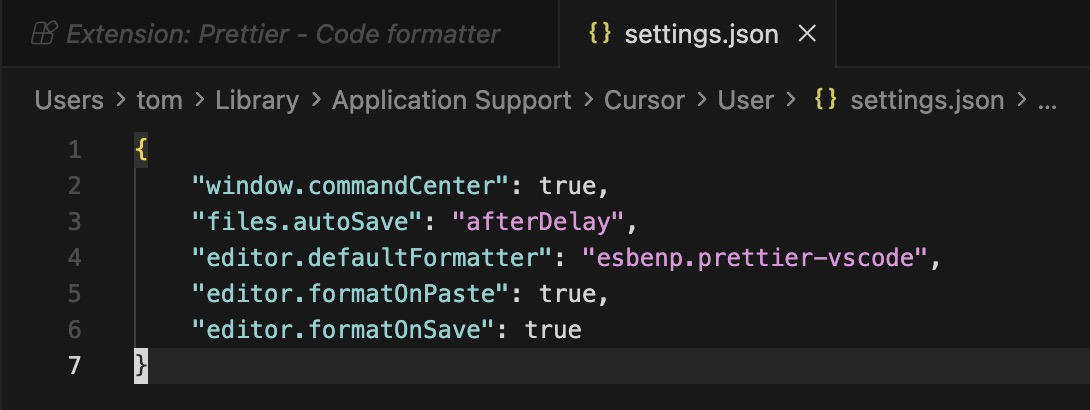
\includegraphics[width=0.8\textwidth]{./assets/img10.jpg}
  \caption{formatOnPaste và formatOnSave}
  \label{fig:settingsjson}
\end{figure}

Cấu hình Eslint bằng lệnh \texttt{npx eslint -{}-init}

\begin{figure}[H]
  \centering
  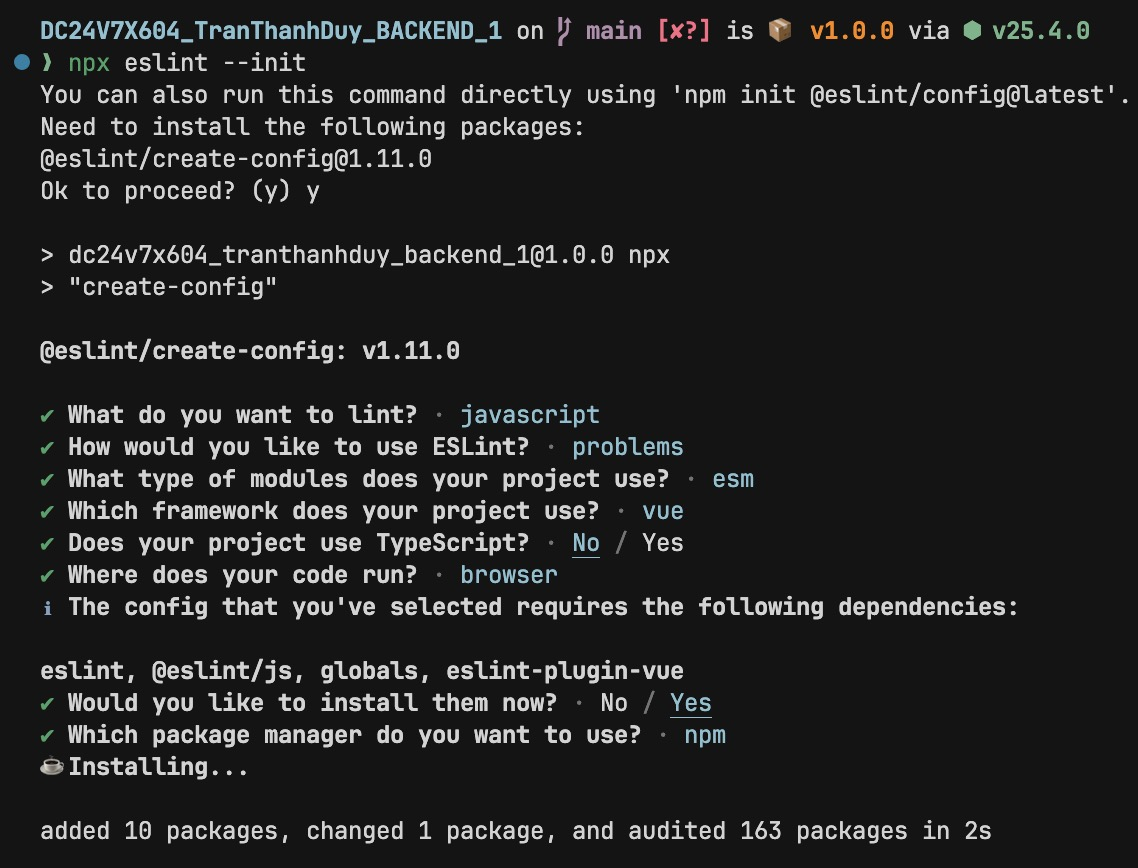
\includegraphics[width=0.6\textwidth]{./assets/img11.jpg}
  \caption{Eslint config}
  \label{fig:eslint_config}
\end{figure}

\section{Cài đặt expressjs}

Tạo tập tin app.js và server.js lần lượt với nội dung sau

Cài đặt app.js

\begin{figure}[H]
    \centering
    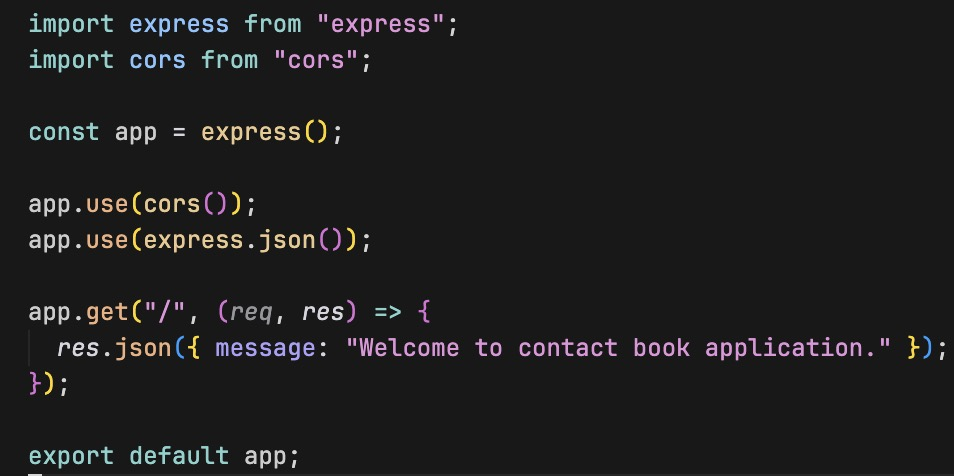
\includegraphics[width=0.8\textwidth]{./assets/img4.jpg}
    \caption{Cài đặt app.js}
    \label{fig:appjs}
\end{figure}

Cài đặt server.js

\begin{figure}[H]
  \centering
  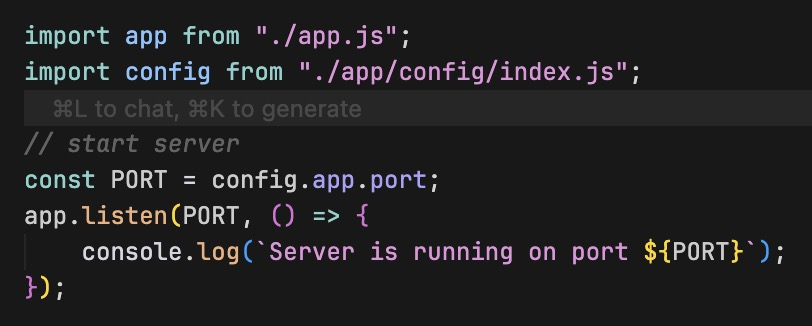
\includegraphics[width=0.8\textwidth]{./assets/img5.jpg}
  \caption{Cài đặt server.js}
  \label{fig:serverjs}
\end{figure}

Lần lượt tạo thư mục app, app/config và tập tin app/config/index.js.

\begin{figure}[H]
  \centering
  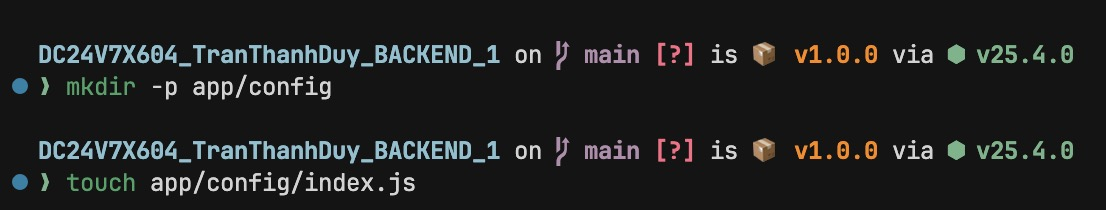
\includegraphics[width=0.8\textwidth]{./assets/img6.jpg}
  \caption{Cài đặt app/config}
  \label{fig:appconfig}
\end{figure}

Cài đặt index.js

\begin{figure}[H]
  \centering
  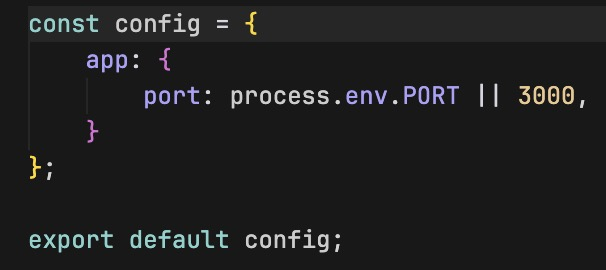
\includegraphics[width=0.8\textwidth]{./assets/img7.jpg}
  \caption{Cài đặt index.js}
  \label{fig:indexjs}
\end{figure}

Kiểm thử hoạt động của Node server

Dùng lệnh \texttt{node server.js}

\begin{figure}[H]
  \centering
  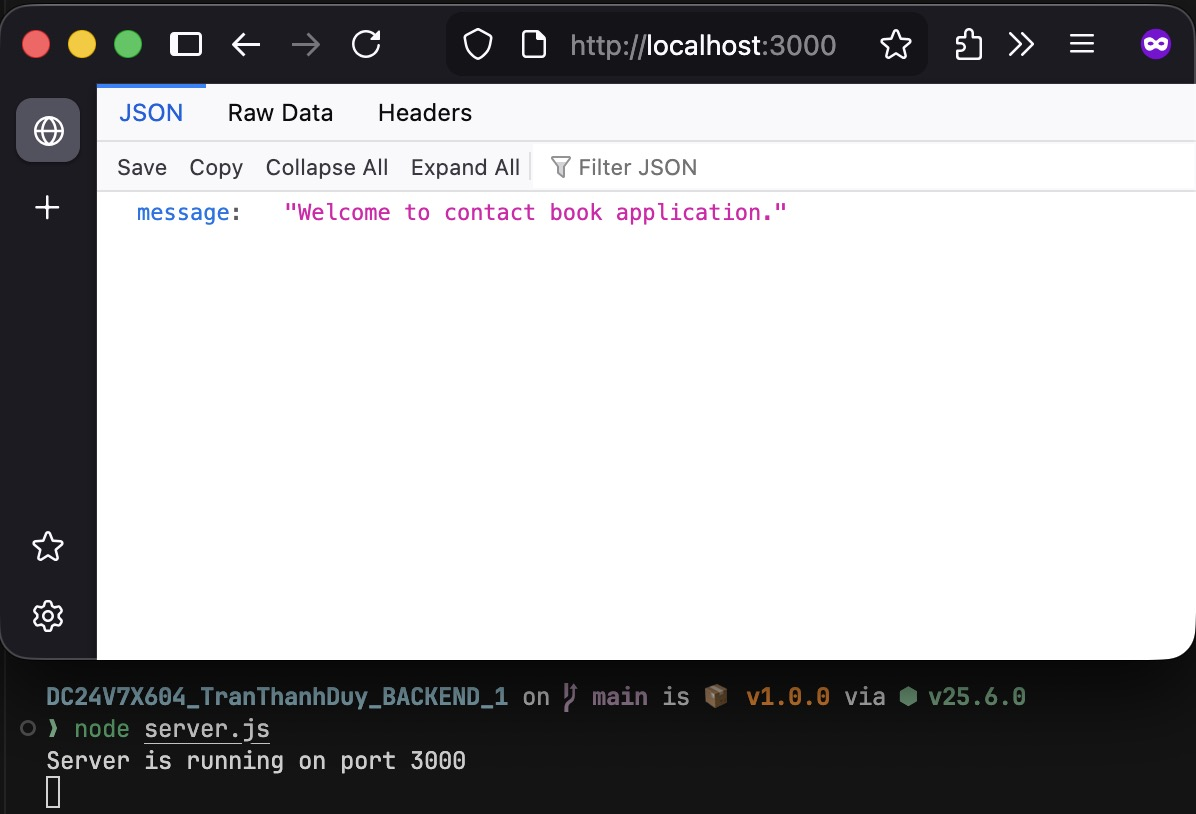
\includegraphics[width=0.8\textwidth]{./assets/img12.jpg}
  \caption{Node Server}
  \label{fig:nodeserver}
\end{figure}


\section{Định nghĩa controllers và các route }

Tạo thư mục app/controllers và tập tin app/controllers/index.js.

\begin{figure}[H]
  \centering
  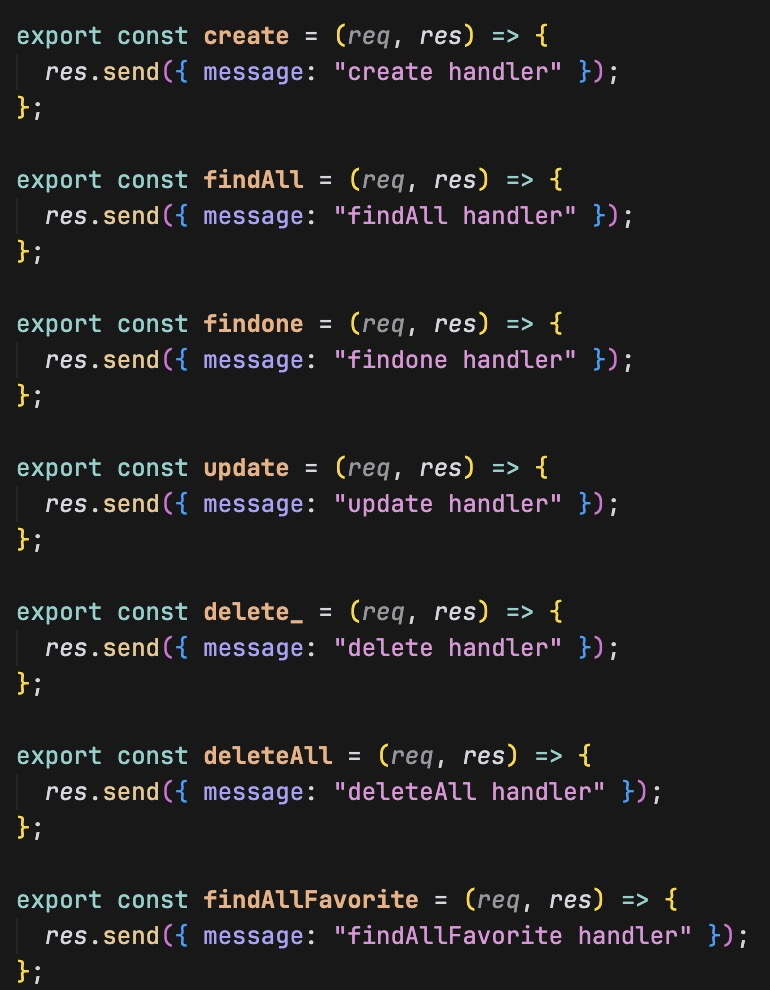
\includegraphics[width=0.5\textwidth]{./assets/img13.jpg}
  \caption{Cài đặt app/controllers/index.js}
  \label{fig:appcontrollers}
\end{figure}

Tạo thư mục app/routes và tập tin app/routes/index.js.

\begin{figure}[H]
  \centering
  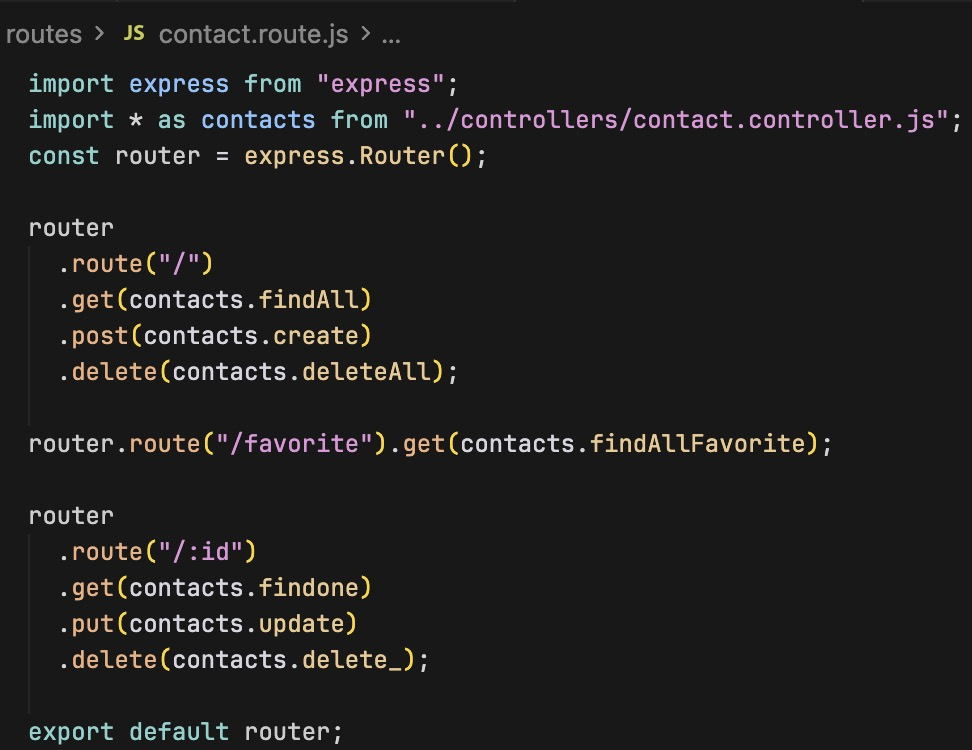
\includegraphics[width=0.8\textwidth]{./assets/img14.jpg}
  \caption{Cài đặt app/routes/index.js}
  \label{fig:approutes}
\end{figure}

Chỉnh sửa app.js với nội dung sau đây

\begin{lstlisting}
...
import contactsRoute from "./app/routes/contact.route.js";

...
app.use("/api/contacts", contactsRoute);
export default app;
\end{lstlisting}

% \begin{figure}[H]
%   \centering
%   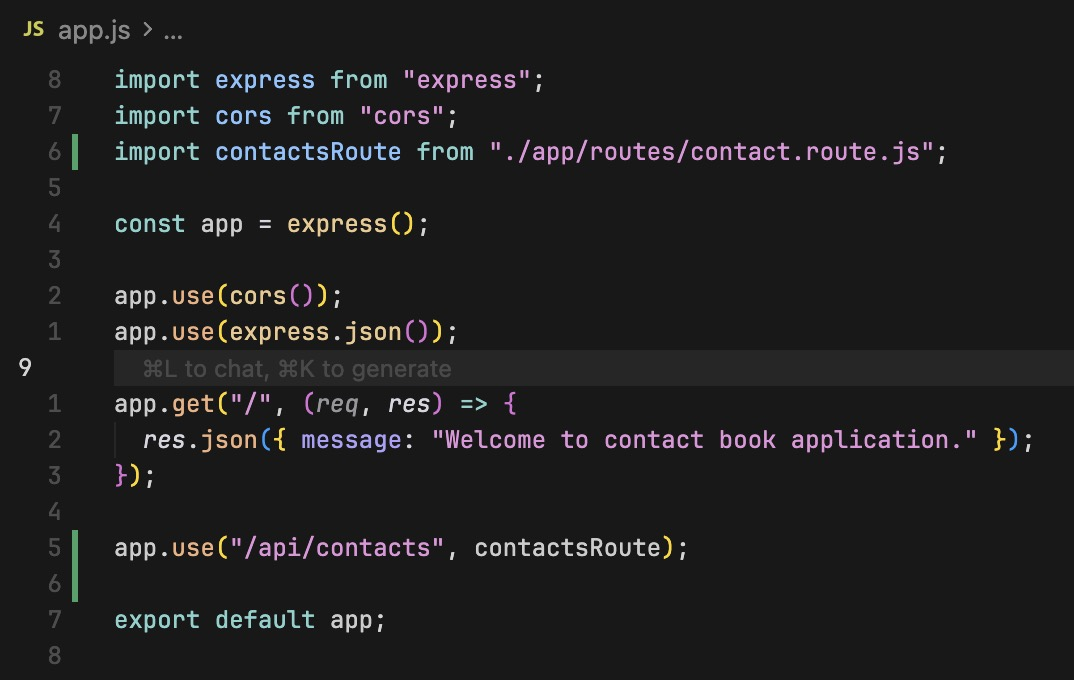
\includegraphics[width=0.8\textwidth]{./assets/img15.jpg}
%   \caption{Chỉnh sửa app.js}
%   \label{fig:appjs_chinhsua}
% \end{figure}

Kiểm thử API bằng phần mềm Postman

\begin{figure}[H]
  \centering
  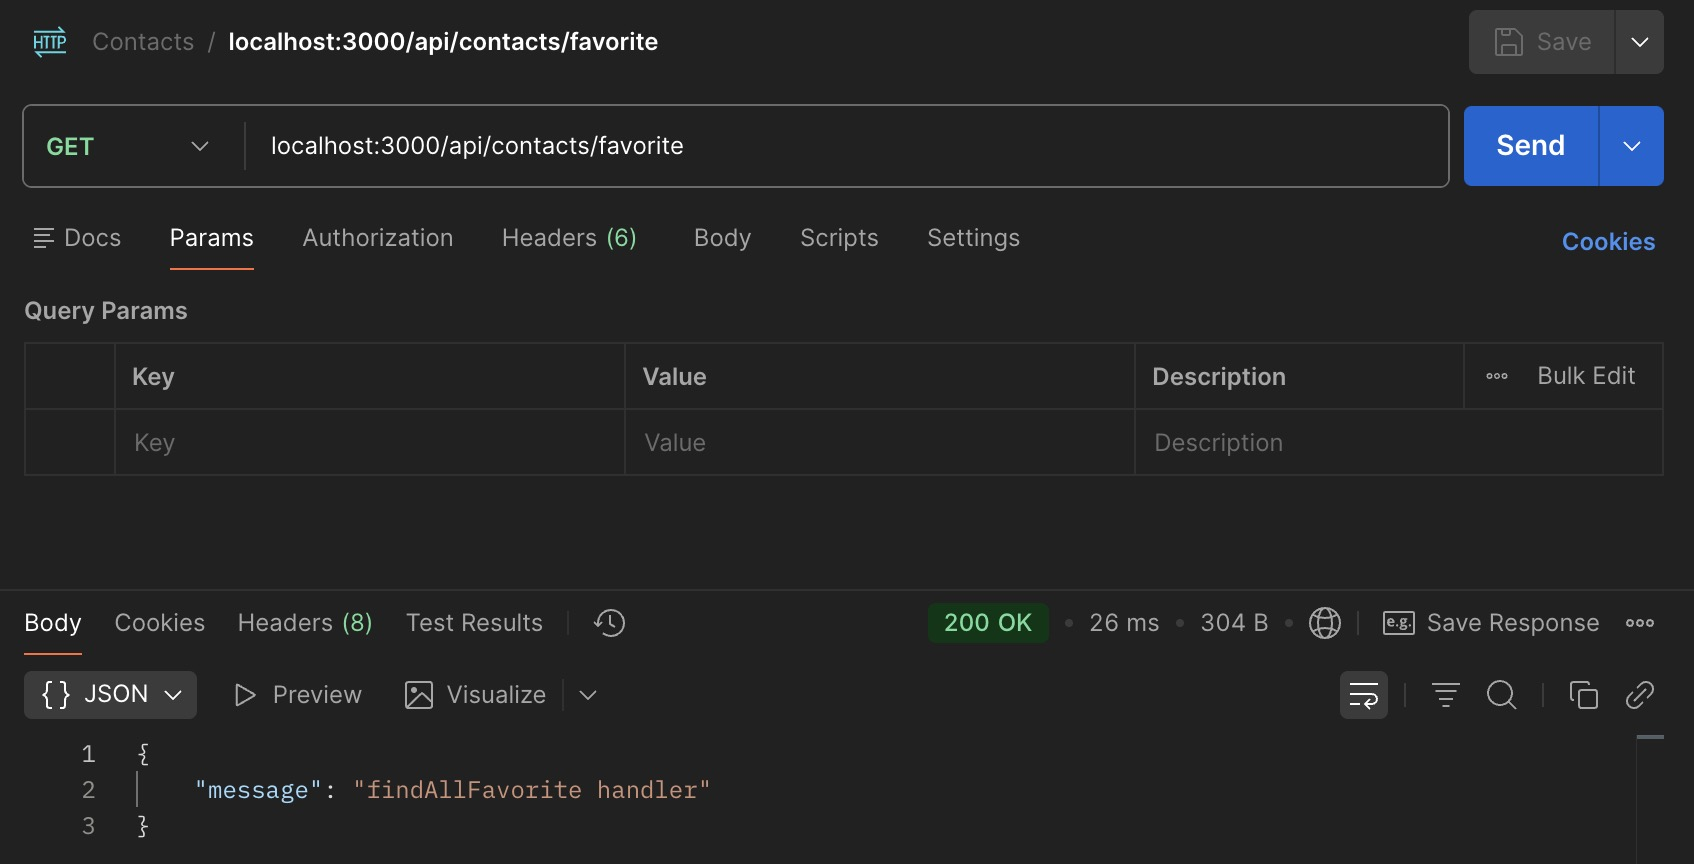
\includegraphics[width=0.8\textwidth]{./assets/img16.jpg}
  \caption{Postman GET /api/contacts/favorite}
  \label{fig:postman}
\end{figure}

\section{Cài đặt xử lý lỗi app/api-error.js}

\begin{figure}[H]
  \centering
  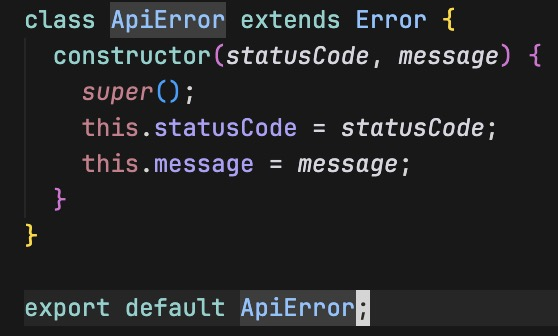
\includegraphics[width=0.8\textwidth]{./assets/img17.jpg}
  \caption{Cài đặt app/api-error.js}
  \label{fig:apierror}
\end{figure}

Chỉnh sửa app.js
\begin{lstlisting}
...
import ApiError from "./app/api-error.js";  
...
// handle 404 error
app.use((req, res, next) => {
  return next(new ApiError(404, "Resource not found"));
});

// define error-handling middleware last, after other app.use() and routes calls
app.use((err, req, res, next) => {
  return res.status(err.statusCode || 500).json({
    message: err.message || "Internal Server Error",
  });
}); 
\end{lstlisting}

\section{Cấu trúc thư mục dự án đến thời điểm này}

\begin{figure}[H]
  \centering
  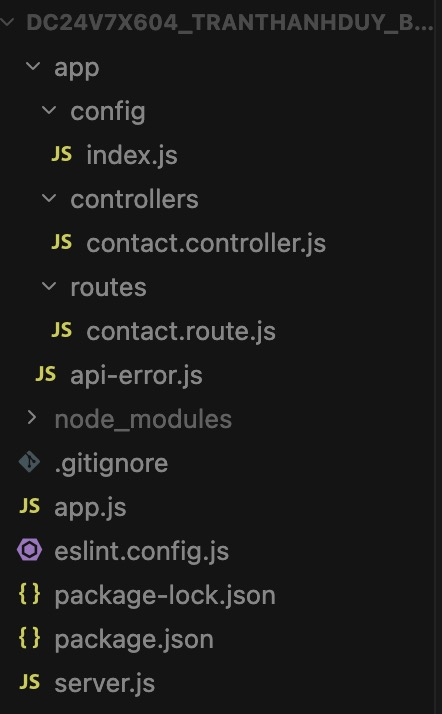
\includegraphics[width=0.4\textwidth]{./assets/img18.jpg}
  \caption{Cấu trúc thư mục dự án}
  \label{fig:project_structure}
\end{figure}

\section{Link Github}

\url{https://github.com/duytechie/DC24V7X604_TranThanhDuy_BACKEND_1}




% CHAPTER 2
\chapter{BACKEND 2}
\section{Cài đặt MongoDB}

Cài đặt MongoDB server bằng docker compose.

\begin{figure}[H]
  \centering
  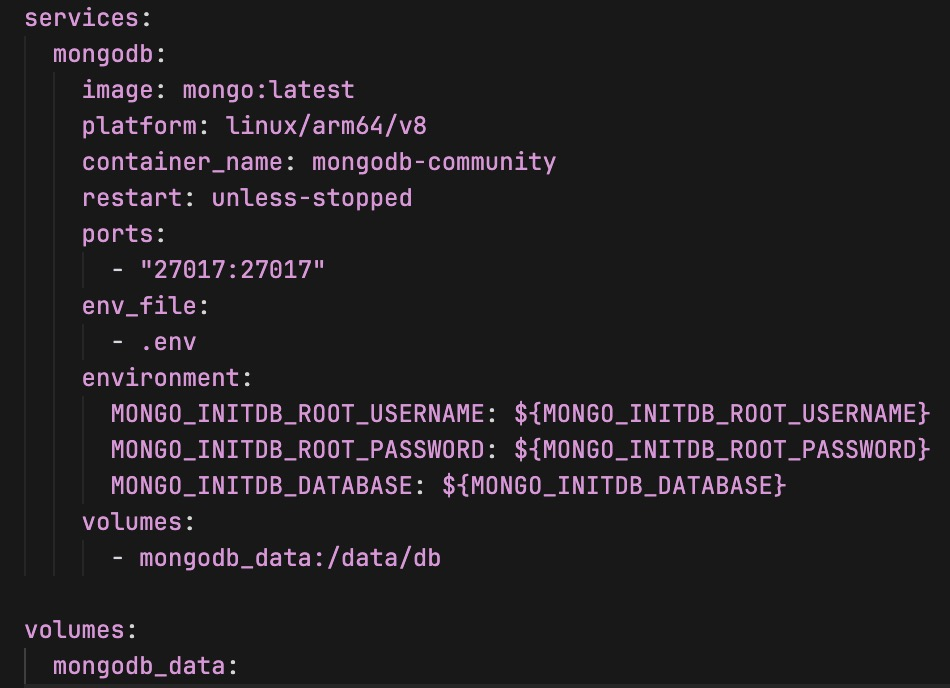
\includegraphics[width=0.8\textwidth]{./assets/img19.jpg}
  \caption{Cài đặt MongoDB server}
  \label{fig:mongodb}
\end{figure}

Chạy lệnh \texttt{docker-compose up -d} để khởi động MongoDB.

Kết nối MongoDB bằng phần mềm MongoDB Compass.

\begin{figure}[H]
  \centering
  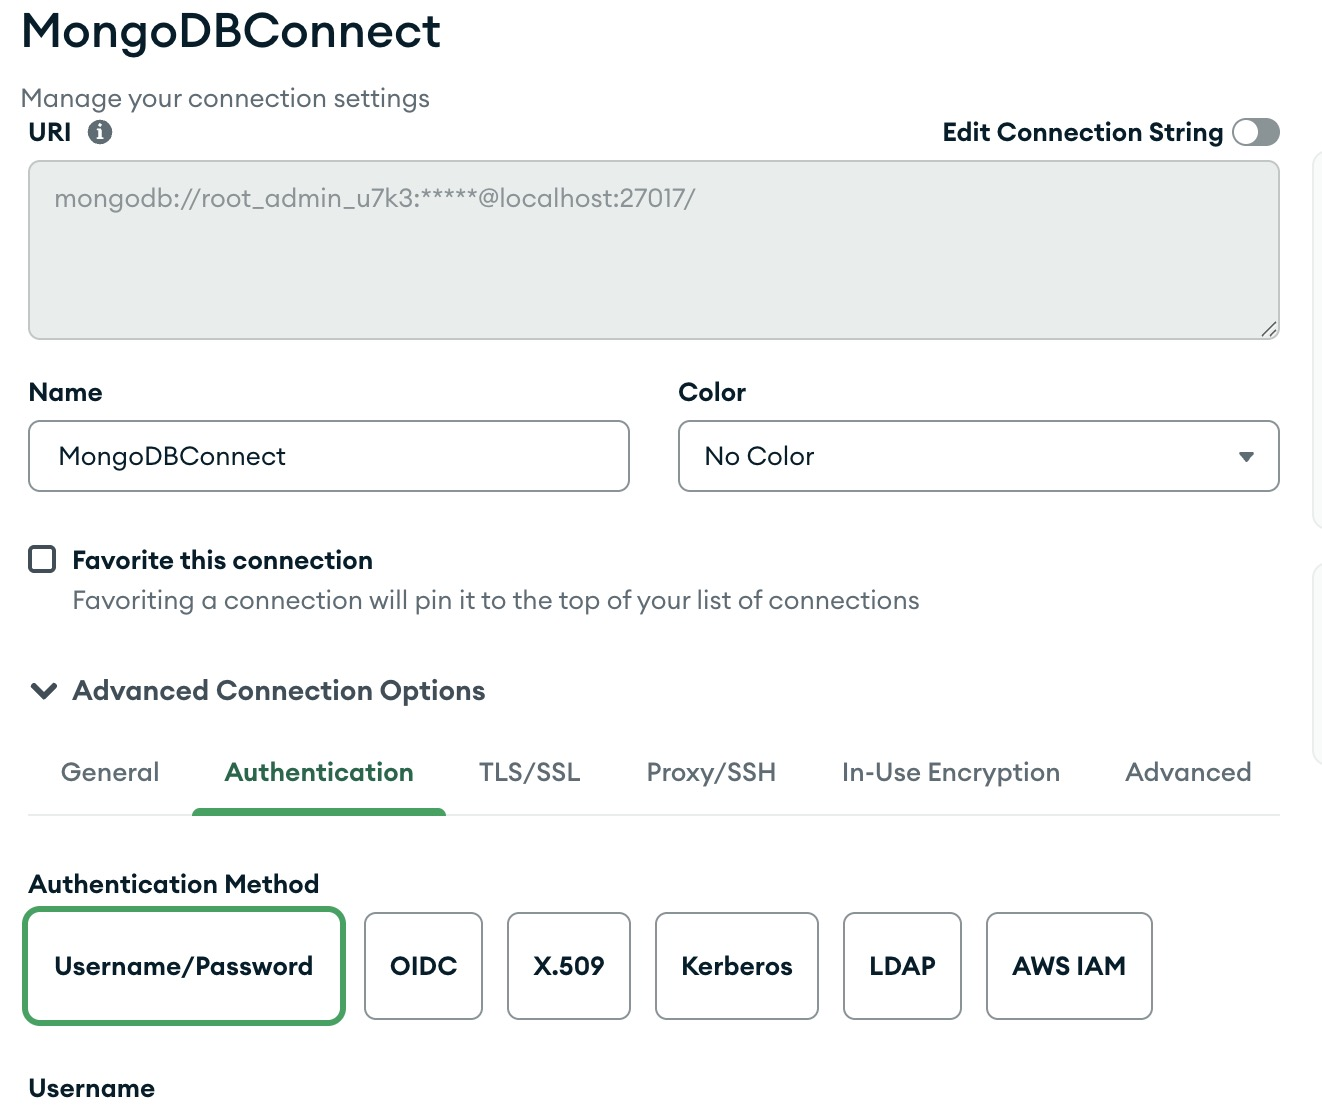
\includegraphics[width=0.8\textwidth]{./assets/img20.jpg}
  \caption{Kết nối MongoDB}
  \label{fig:mongodb_compass}
\end{figure}

\section{Thiết lập cấu trúc kết nối cơ sở dữ liệu MongoDB}

Cấu hình (app/config/index.js)

\begin{figure}[H]
  \centering
  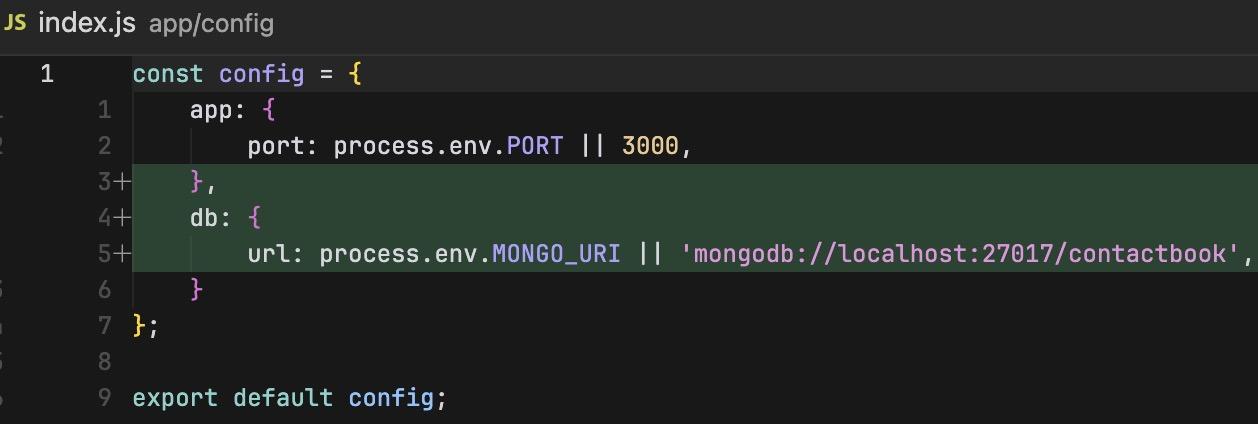
\includegraphics[width=0.8\textwidth]{./assets/img21.jpg}
  \caption{Cấu hình index.js}
  \label{fig:appconfigindexjs}
\end{figure}

Thêm hàm kết nối MongoDB (app/utils/mongodb.utils.js)

\begin{figure}[H]
  \centering
  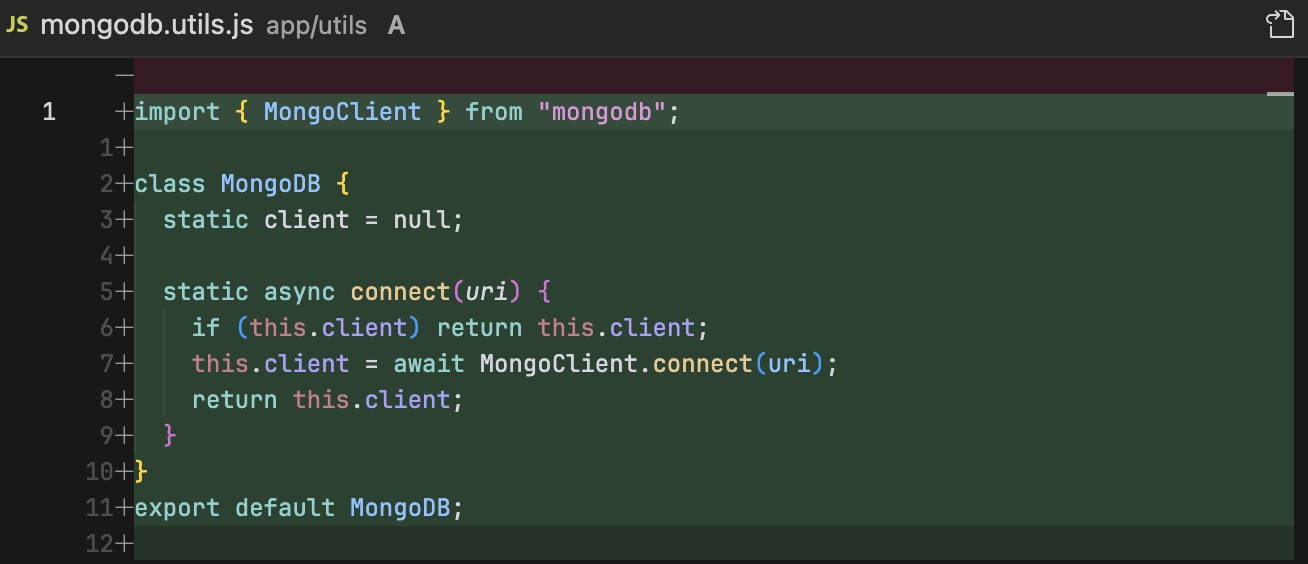
\includegraphics[width=0.8\textwidth]{./assets/img23.jpg}
  \caption{Hàm kết nối MongoDB}
  \label{fig:mongodbutilsjs}
\end{figure}

Cấu hình (app/services/contact.service.js)

\begin{figure}[H]
  \centering
  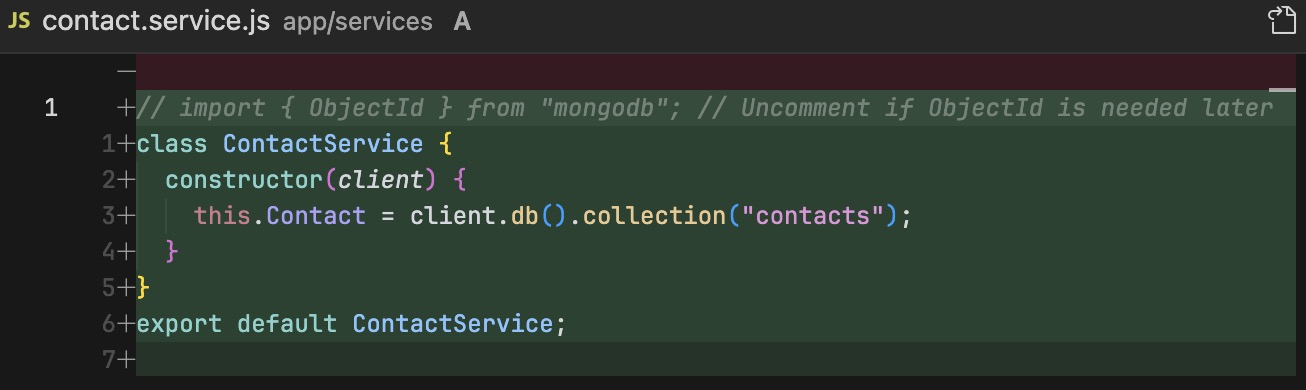
\includegraphics[width=0.8\textwidth]{./assets/img22.jpg}
  \caption{Cấu hình contact.service.js}
  \label{fig:contactservicejs}
\end{figure}

Cấu hình (server.js)

\begin{figure}[H]
  \centering
  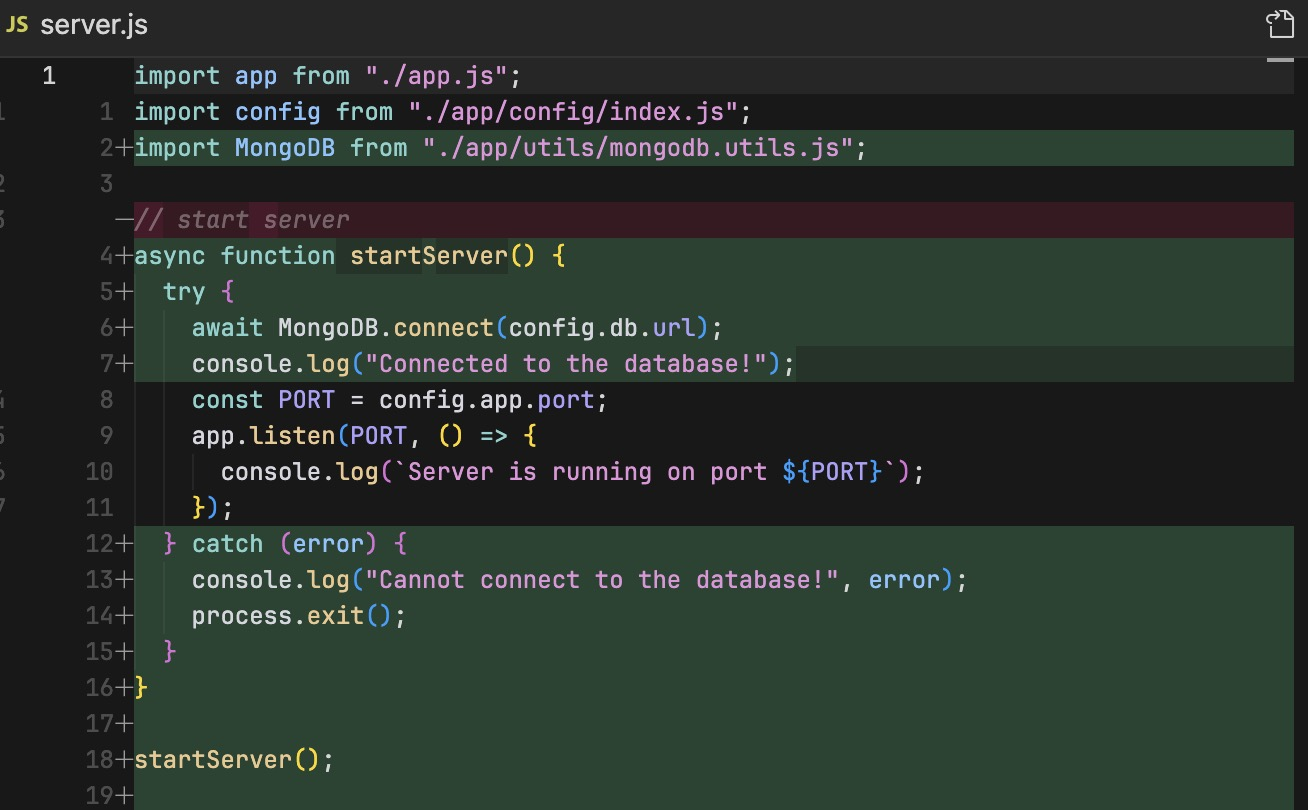
\includegraphics[width=0.8\textwidth]{./assets/img24.jpg}
  \caption{Cấu hình server.js}
  \label{fig:serverjsconfig}
\end{figure}

\section{Cài đặt handler create}

Cấu hình handler create (app/controllers/contact.controller.js)

\begin{figure}[H]
  \centering
  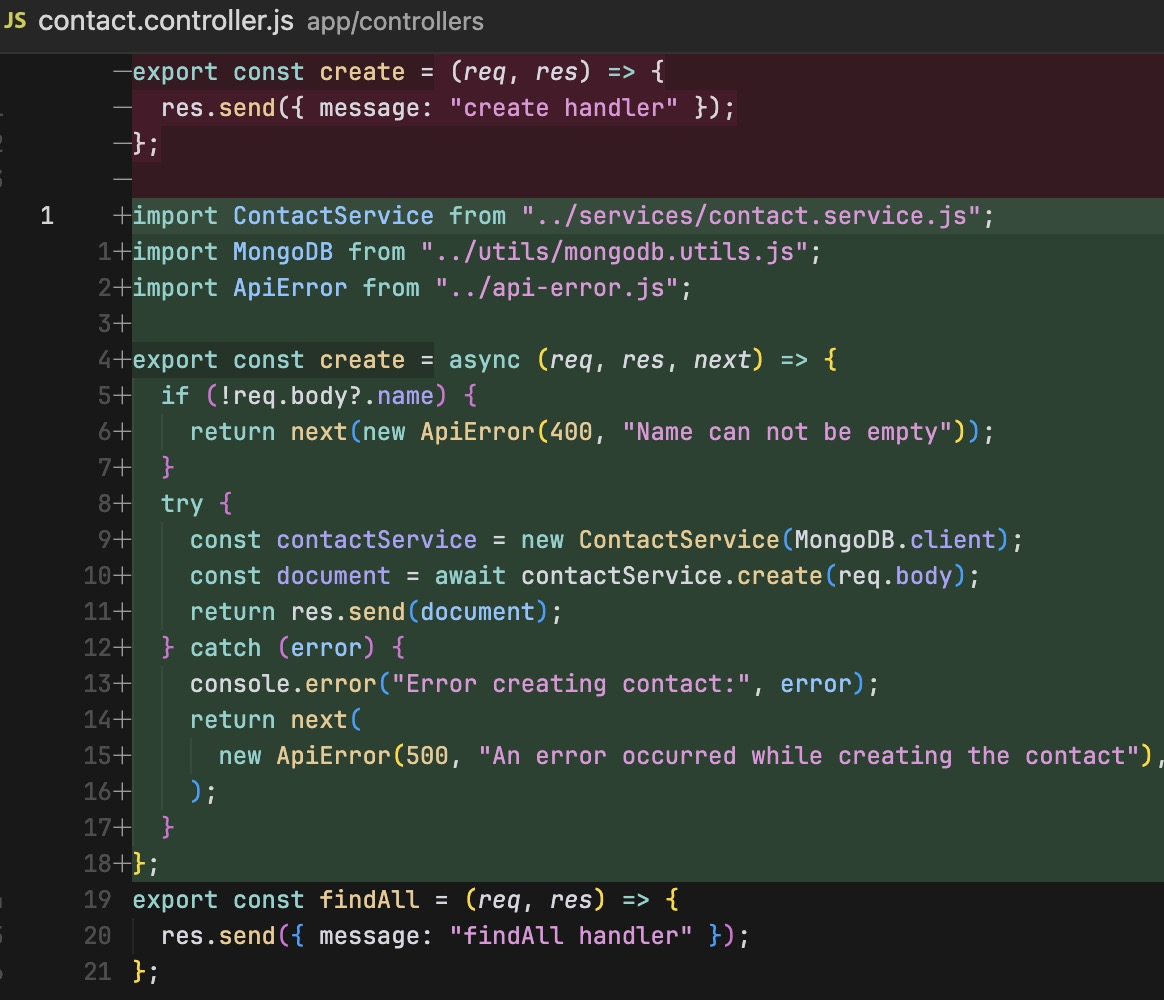
\includegraphics[width=0.8\textwidth]{./assets/contact_controller.jpg}
  \caption{Cấu hình handler create}
  \label{fig:contactcontrollercreate}
\end{figure}

Cấu hình (app/services/contact.service.js)

\begin{figure}[H]
  \centering
  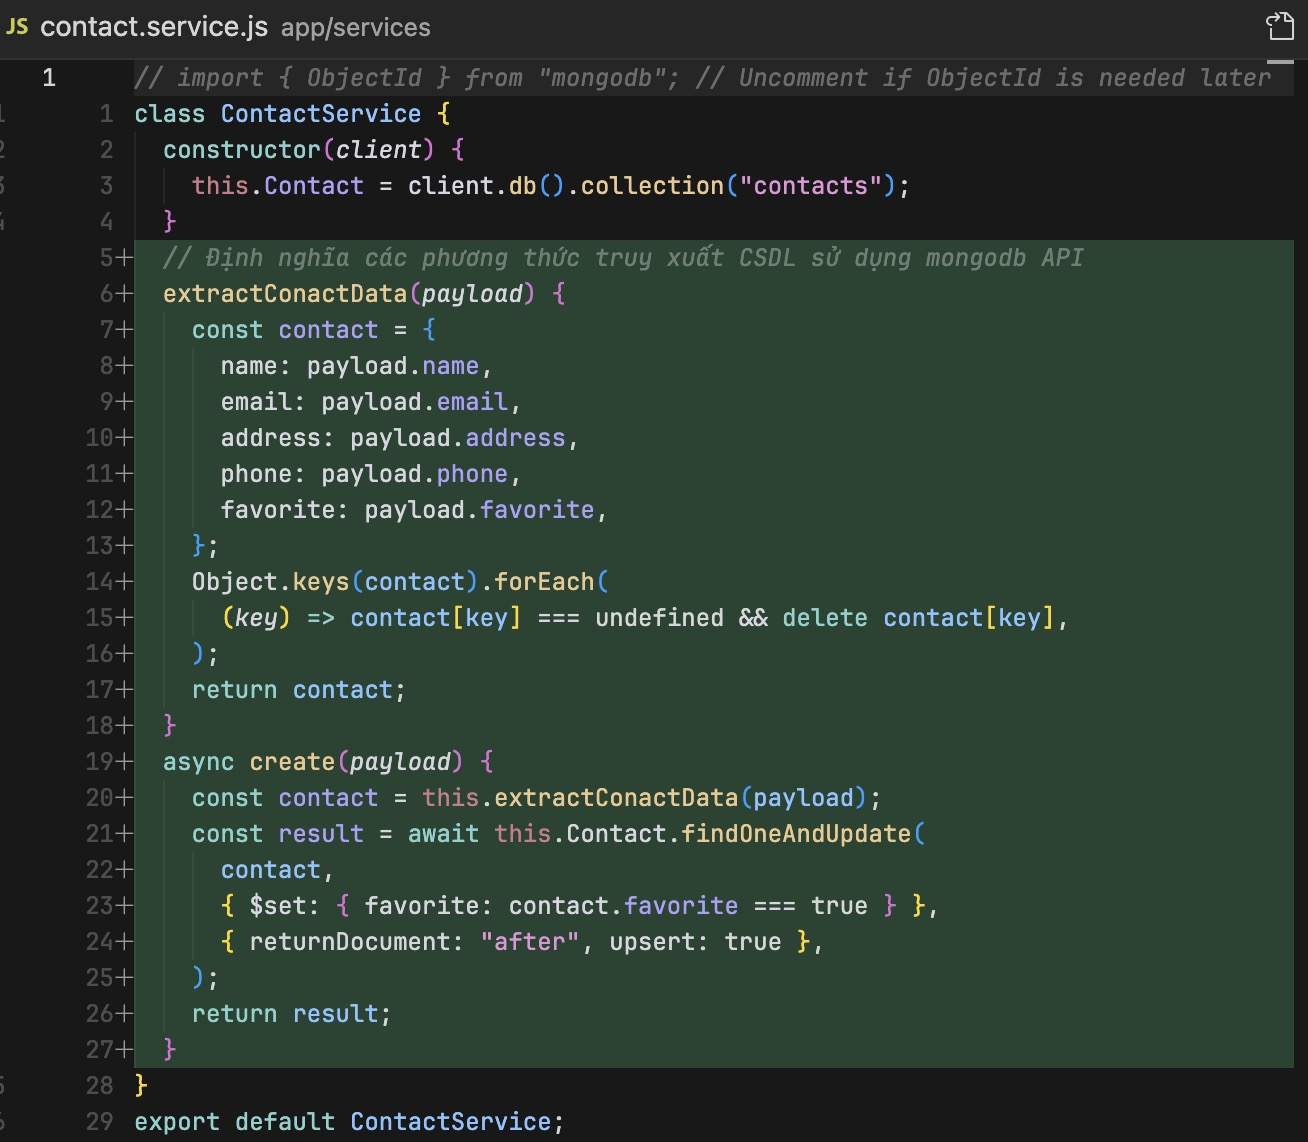
\includegraphics[width=0.8\textwidth]{./assets/contact_service.jpg}
  \caption{Cấu hình contact.service.js}
  \label{fig:contactservicecreate}
\end{figure}


Dùng Postman kiểm tra handler create hoạt động đúng.

\begin{figure}[H]
  \centering
  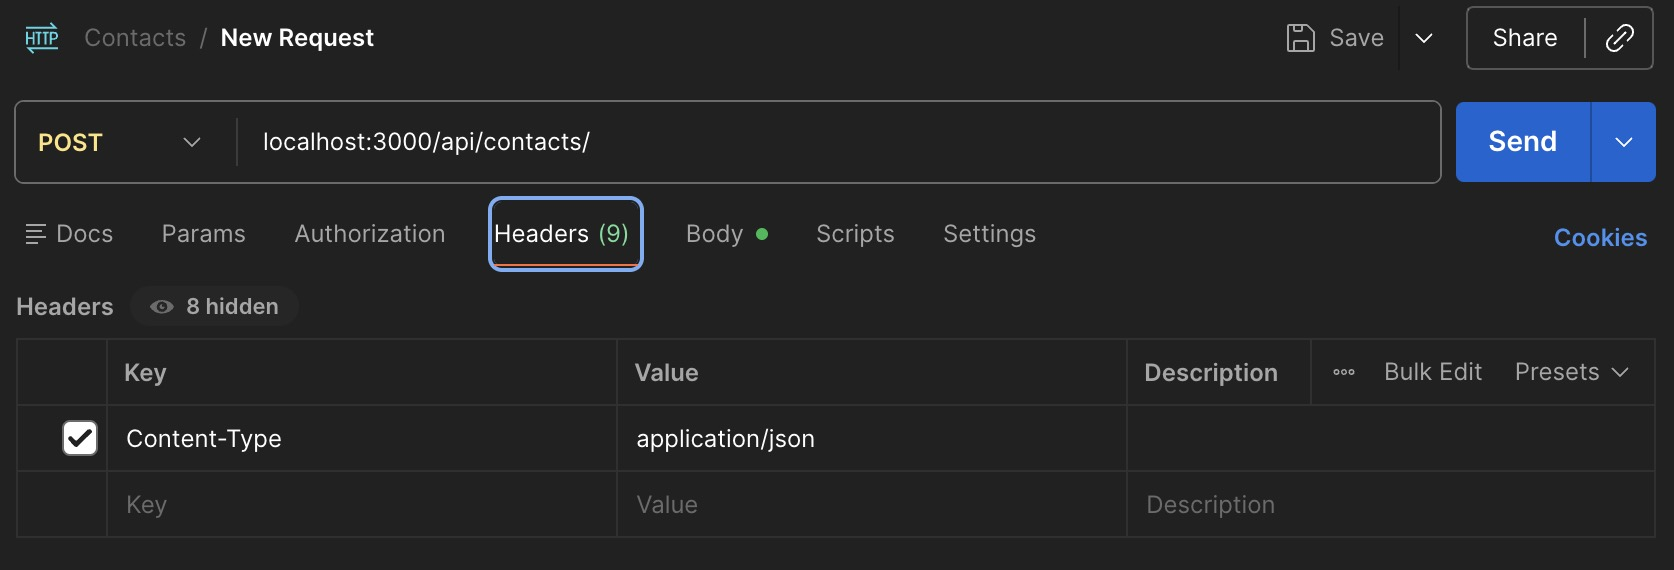
\includegraphics[width=0.8\textwidth]{./assets/img25.jpg}
  \caption{Postman Headers}
  \label{fig:postman_header}
\end{figure}

\begin{figure}[H]
  \centering
  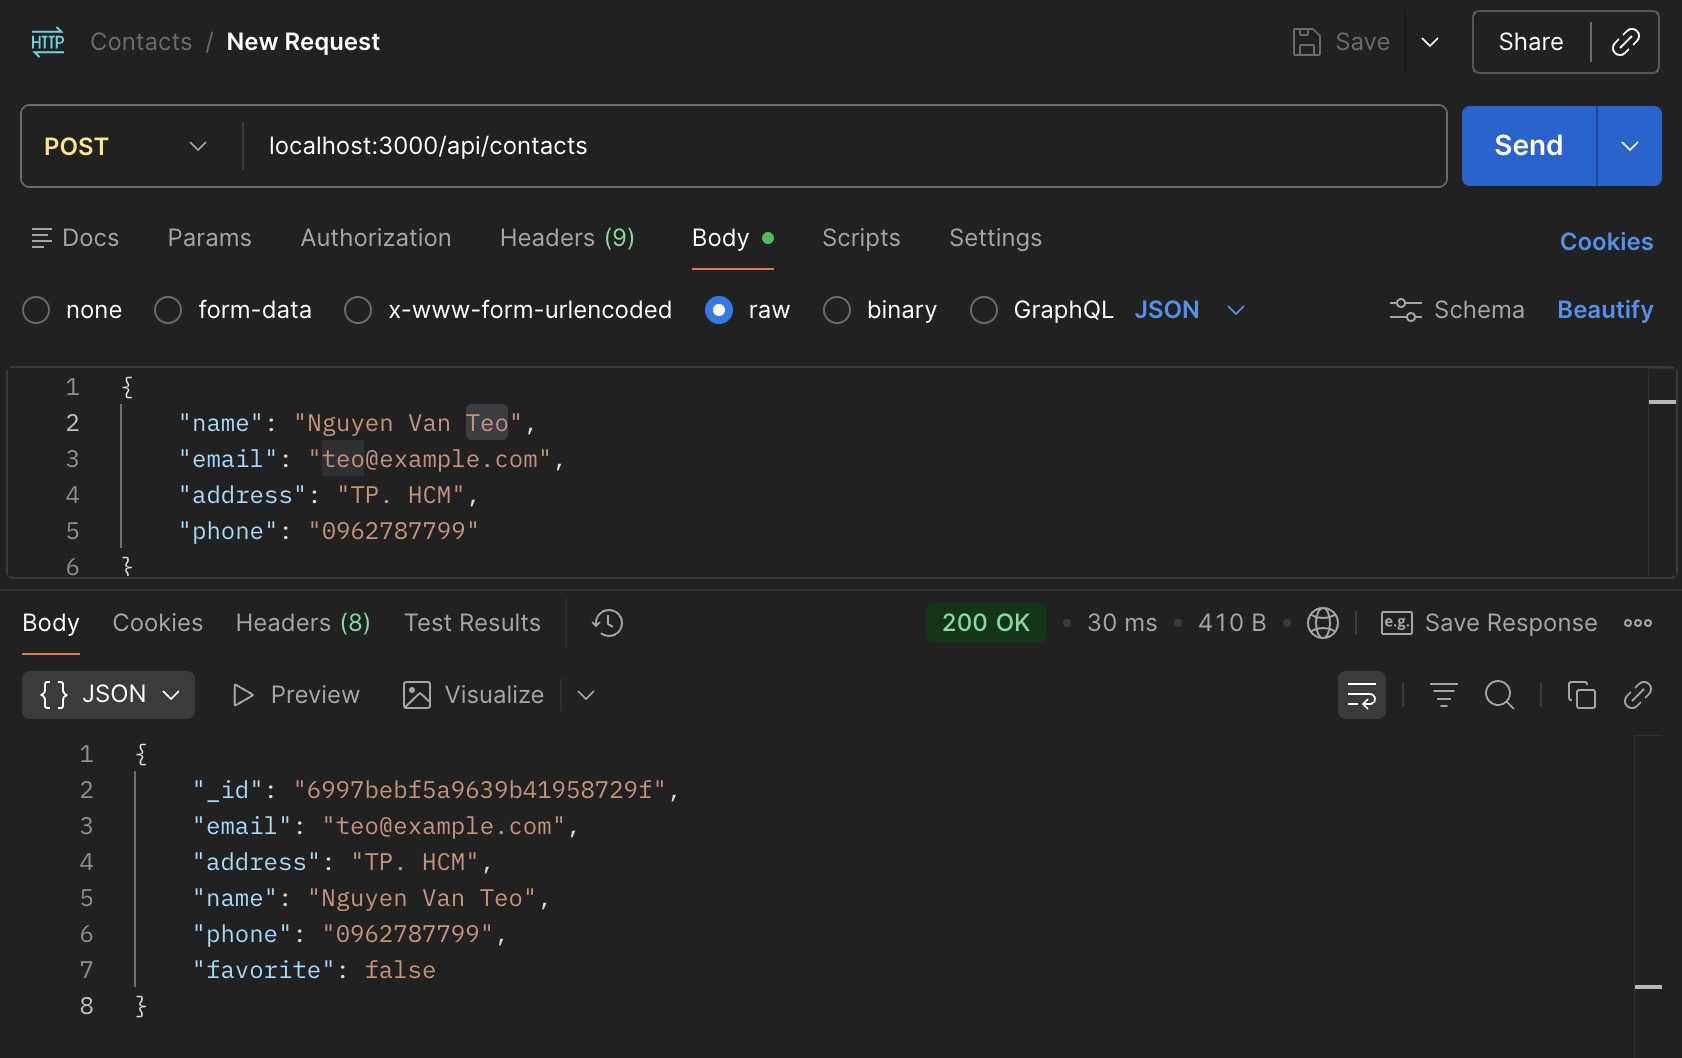
\includegraphics[width=0.8\textwidth]{./assets/img26.jpg}
  \caption{Postman Body}
  \label{fig:postman_body}
\end{figure}

Kiểm tra data được lưu vào MongoDB

\begin{figure}[H]
  \centering
  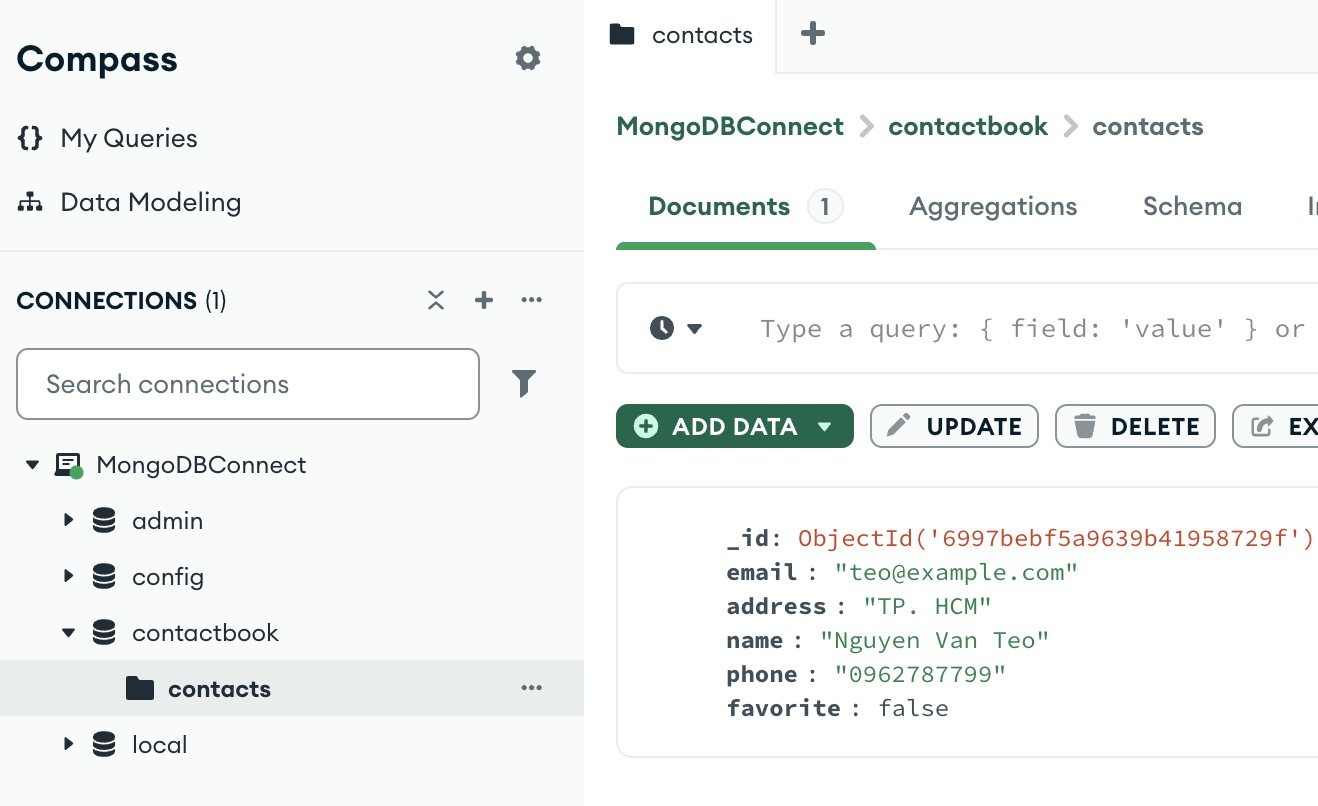
\includegraphics[width=0.8\textwidth]{./assets/img27.jpg}
  \caption{MongoDB Compass}
  \label{fig:mongodb_data}
\end{figure}

\section{Cài đặt handler findAll/findOne }

\begin{figure}[H]
  \centering
  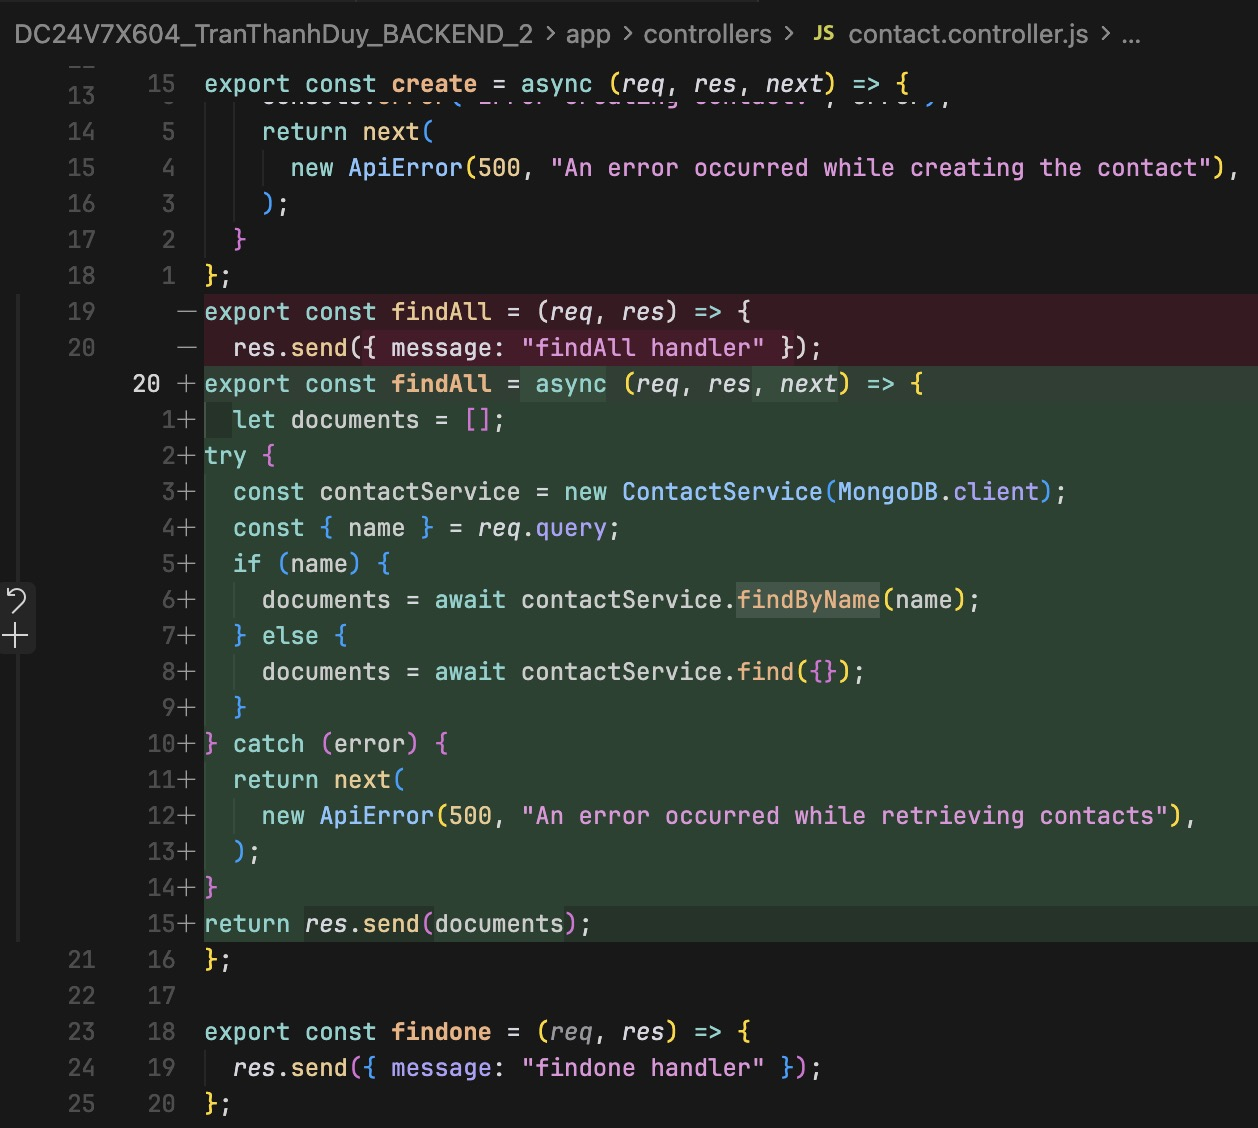
\includegraphics[width=0.8\textwidth]{./assets/handler_findall.jpg}
  \caption{Cài đặt handler findAll}
  \label{fig:contactcontrollerfindall}
\end{figure}

contactService.find(condition) và contactService. findByName(name) lần lượt tìm kiếm các tài liệu thỏa điều
kiện chỉ định trong đối tượng condition, theo tên name. Hai phương thức này có thể được định nghĩa như
sau trong tập tin app/services/contact.service.js.

\begin{figure}[H]
  \centering
  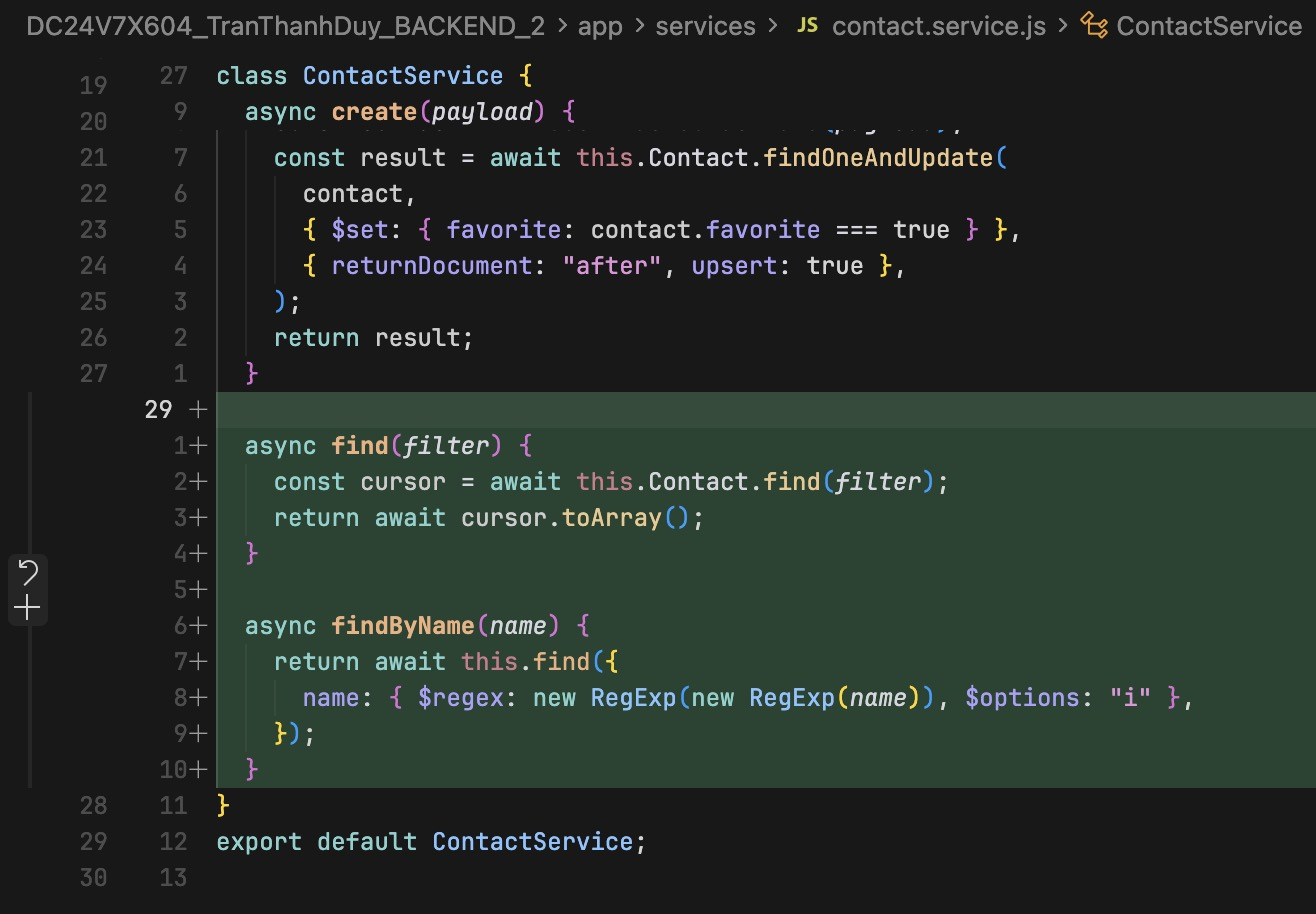
\includegraphics[width=0.8\textwidth]{./assets/find_findbyname_function.jpg}
  \caption{Cài đặt hàm find và findByName}
  \label{fig:find_findbyname_function}
\end{figure}

Dùng Postman kiểm tra handler findAll hoạt động đúng.


\begin{figure}[H]
  \centering
  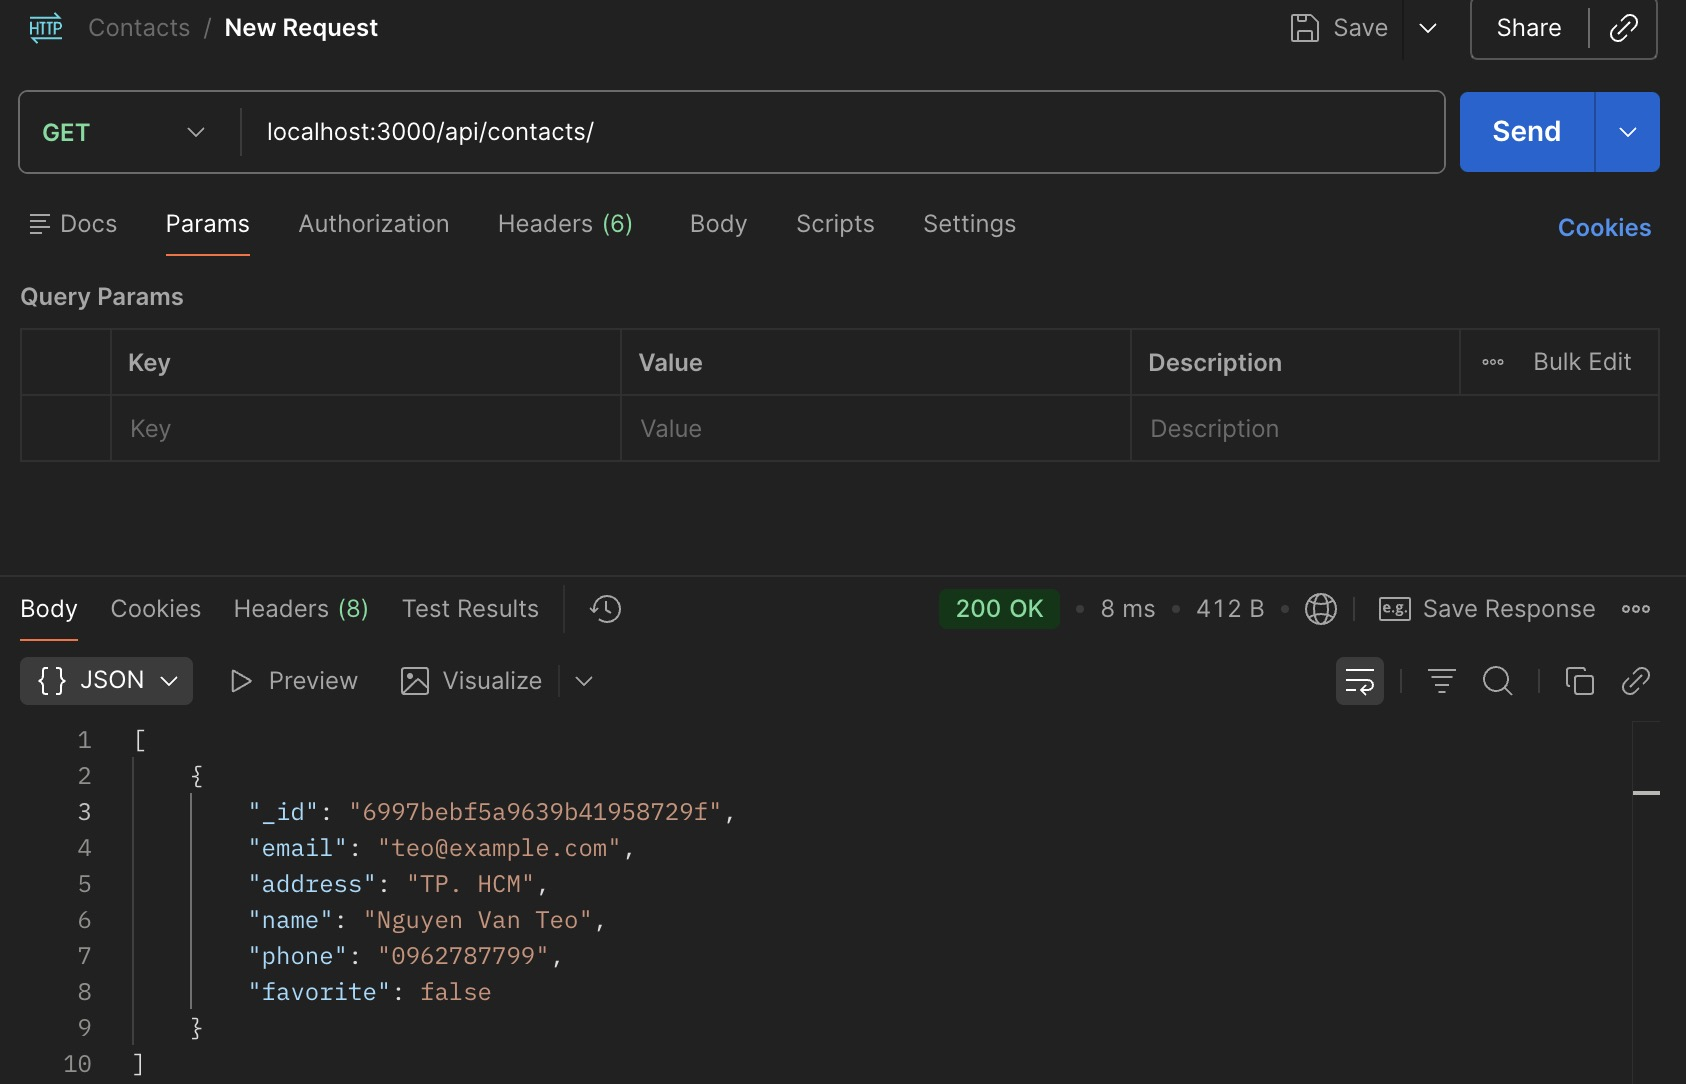
\includegraphics[width=0.8\textwidth]{./assets/postman_findall.jpg}
  \caption{Postman findAll}
  \label{fig:postman_findall}
\end{figure}

Kiểm tra function findByName

\begin{figure}[H]
  \centering
  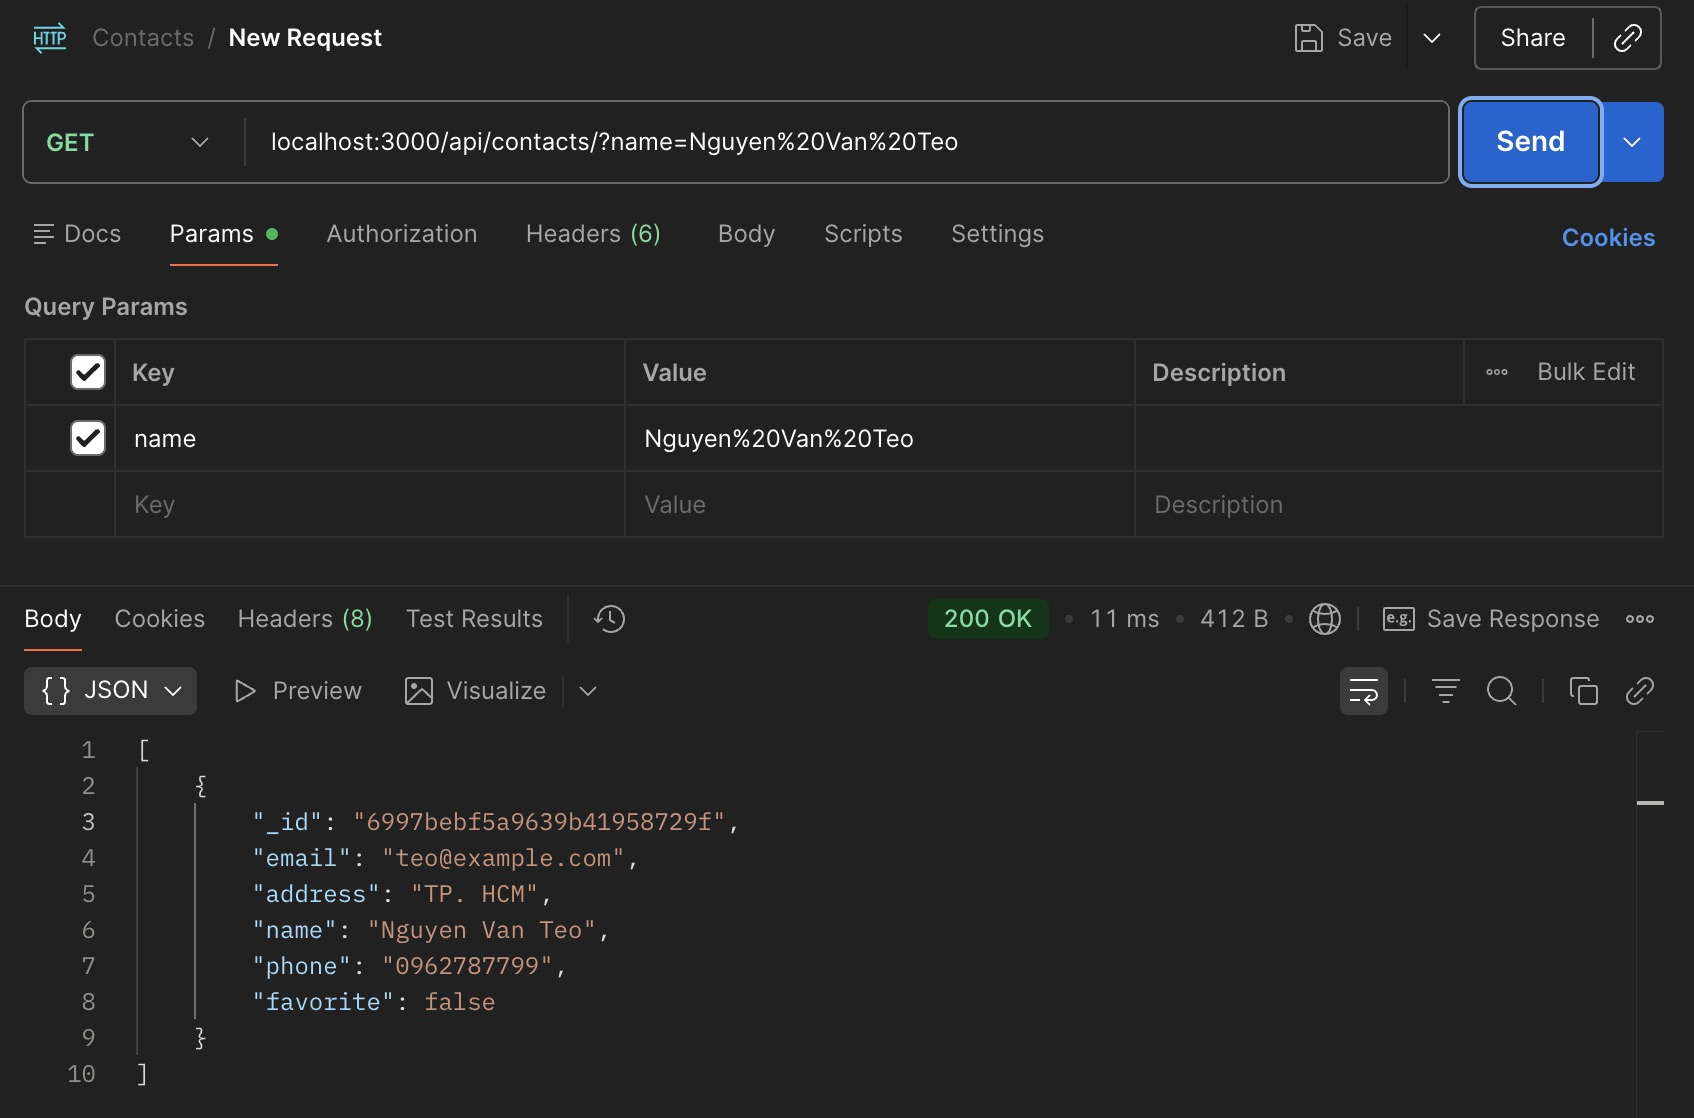
\includegraphics[width=0.8\textwidth]{./assets/postman_findname.jpg}
  \caption{Postman findByName}
  \label{fig:postman_findbyname}
\end{figure}

Cài đặt handler findOne 

\begin{figure}[H]
  \centering
  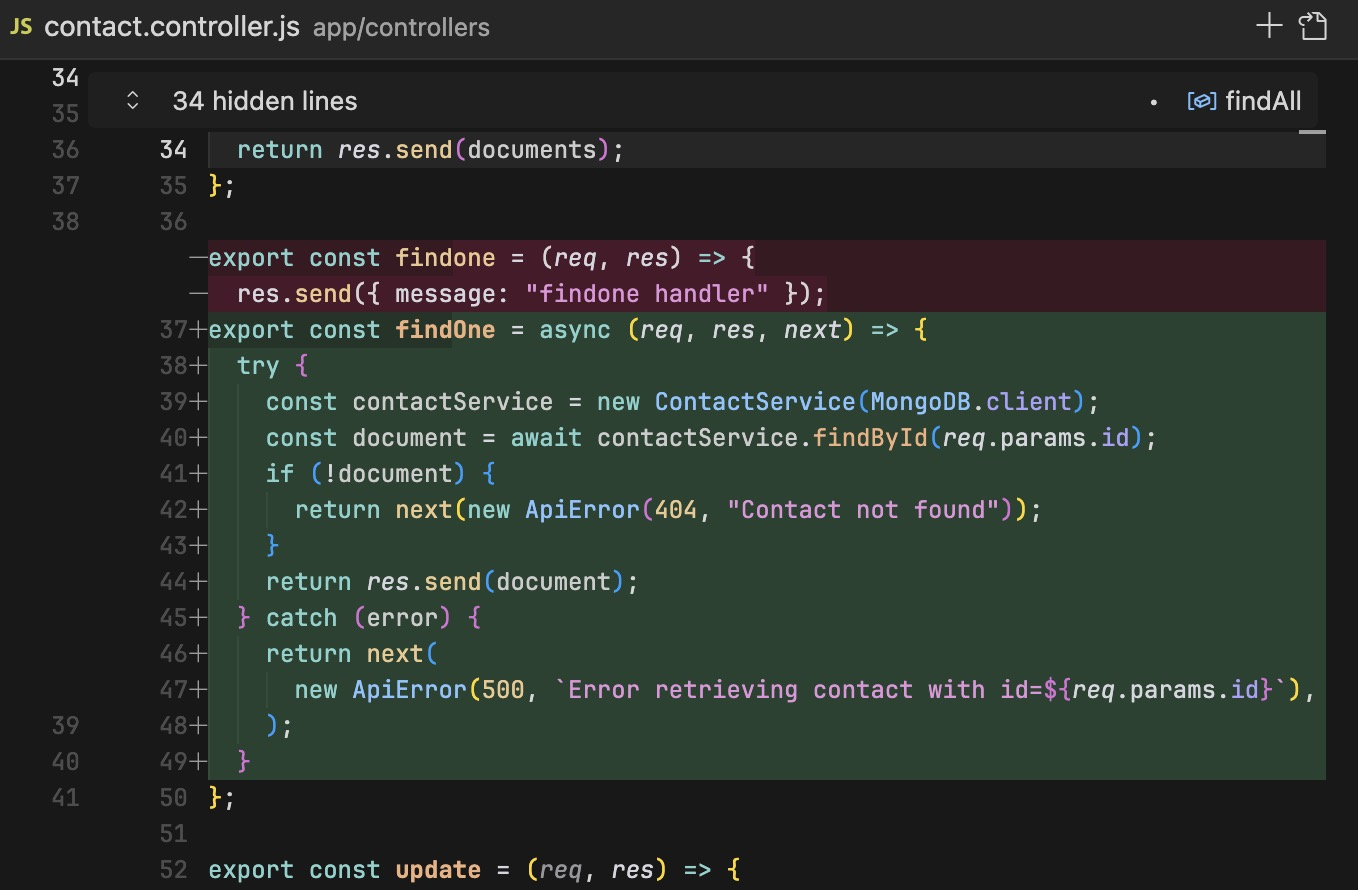
\includegraphics[width=0.8\textwidth]{./assets/handler_findone.jpg}
  \caption{Cài đặt handler findOne}
  \label{fig:contactcontrollerfindone}
\end{figure}

contactService.findByld(id) tìm kiếm tài liệu theo Id. Phương thức findByld(id) có thể được định nghĩa như
sau trong tập tin app/services/contact.service.js.
\begin{figure}[H]
  \centering
  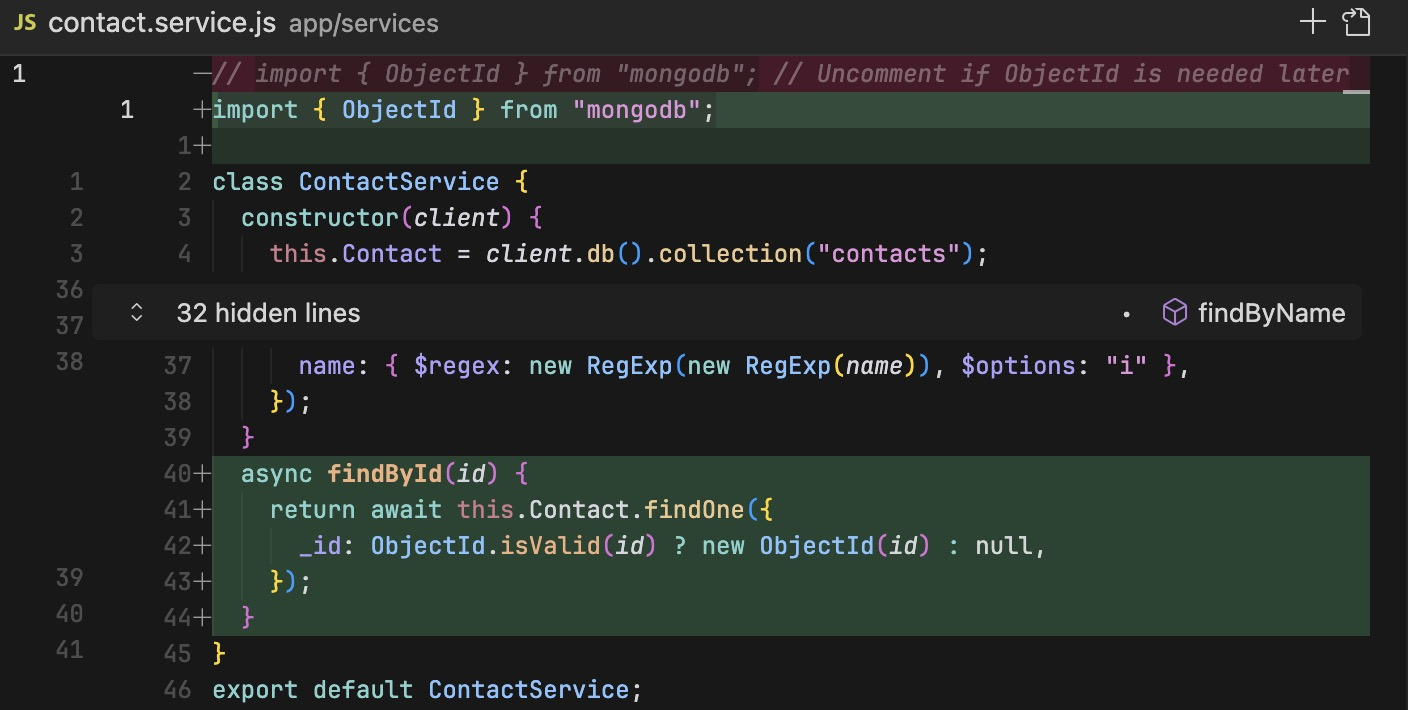
\includegraphics[width=0.8\textwidth]{./assets/findbyid.jpg}
  \caption{Cài đặt hàm findById}
  \label{fig:findbyid_function}
\end{figure}

Dùng Postman kiểm tra handler findOne hoạt động đúng.

\begin{figure}[H]
  \centering
  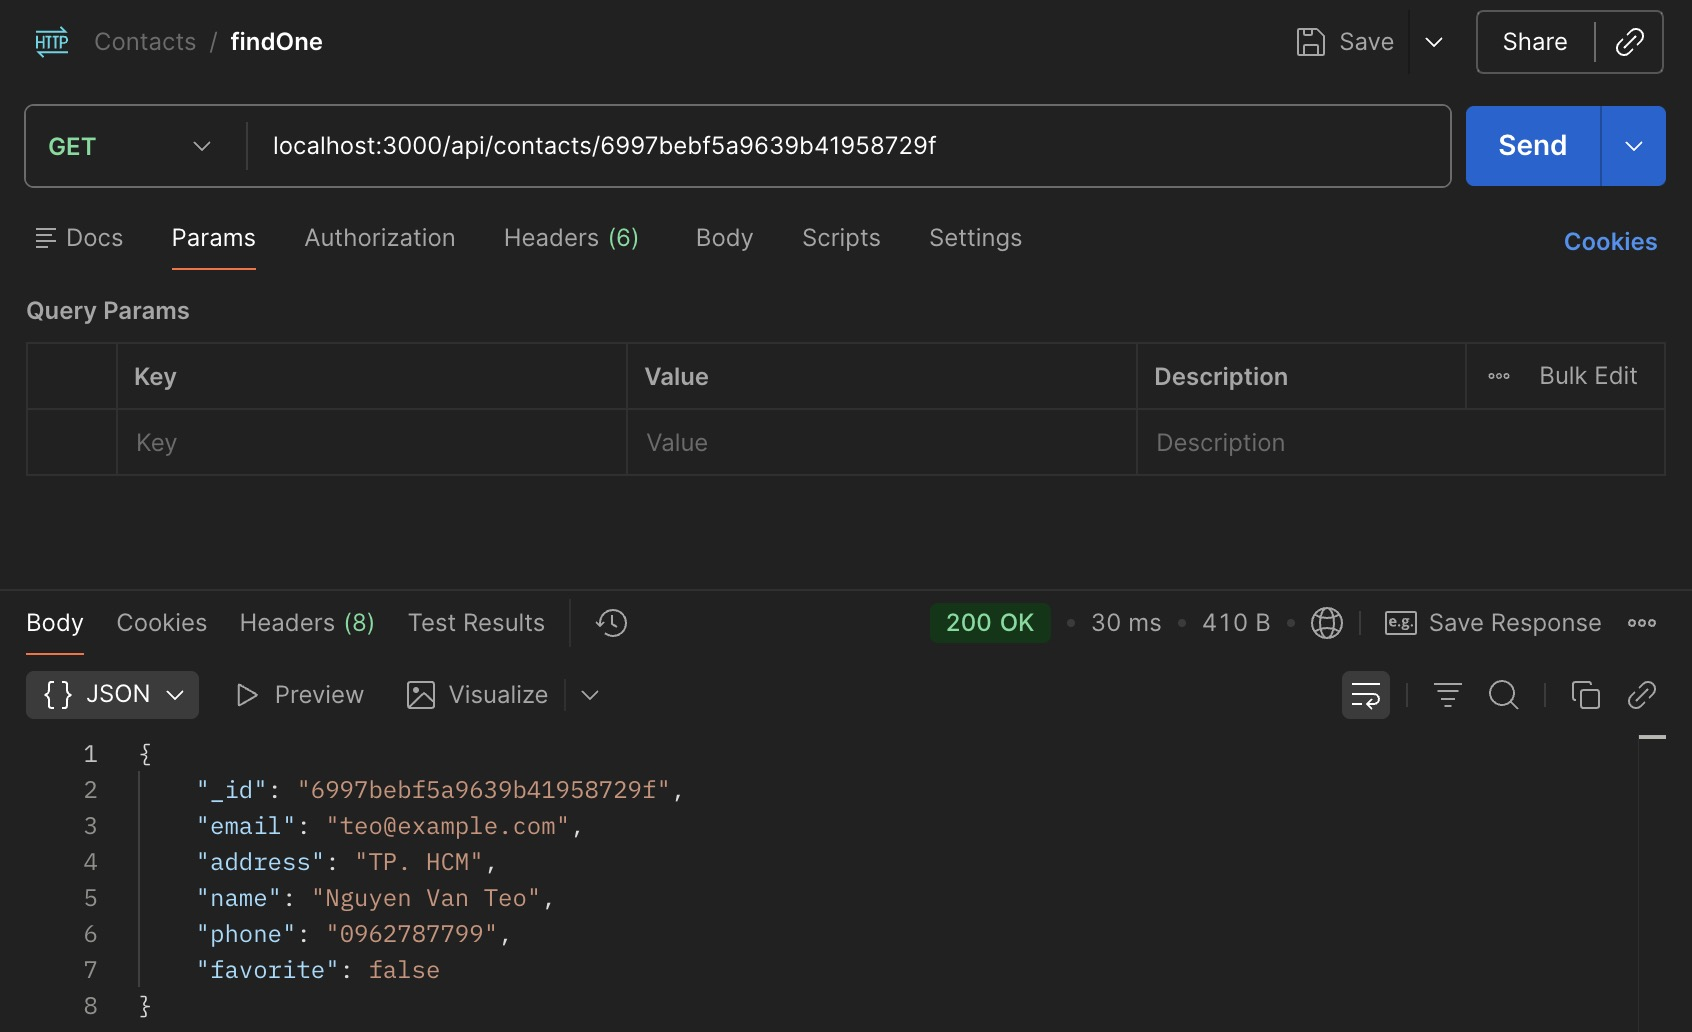
\includegraphics[width=0.8\textwidth]{./assets/postman_findbyid.jpg}
  \caption{Postman findOne}
  \label{fig:postman_findone}
\end{figure}

\section{Cài đặt handler update }

\begin{figure}[H]
  \centering
  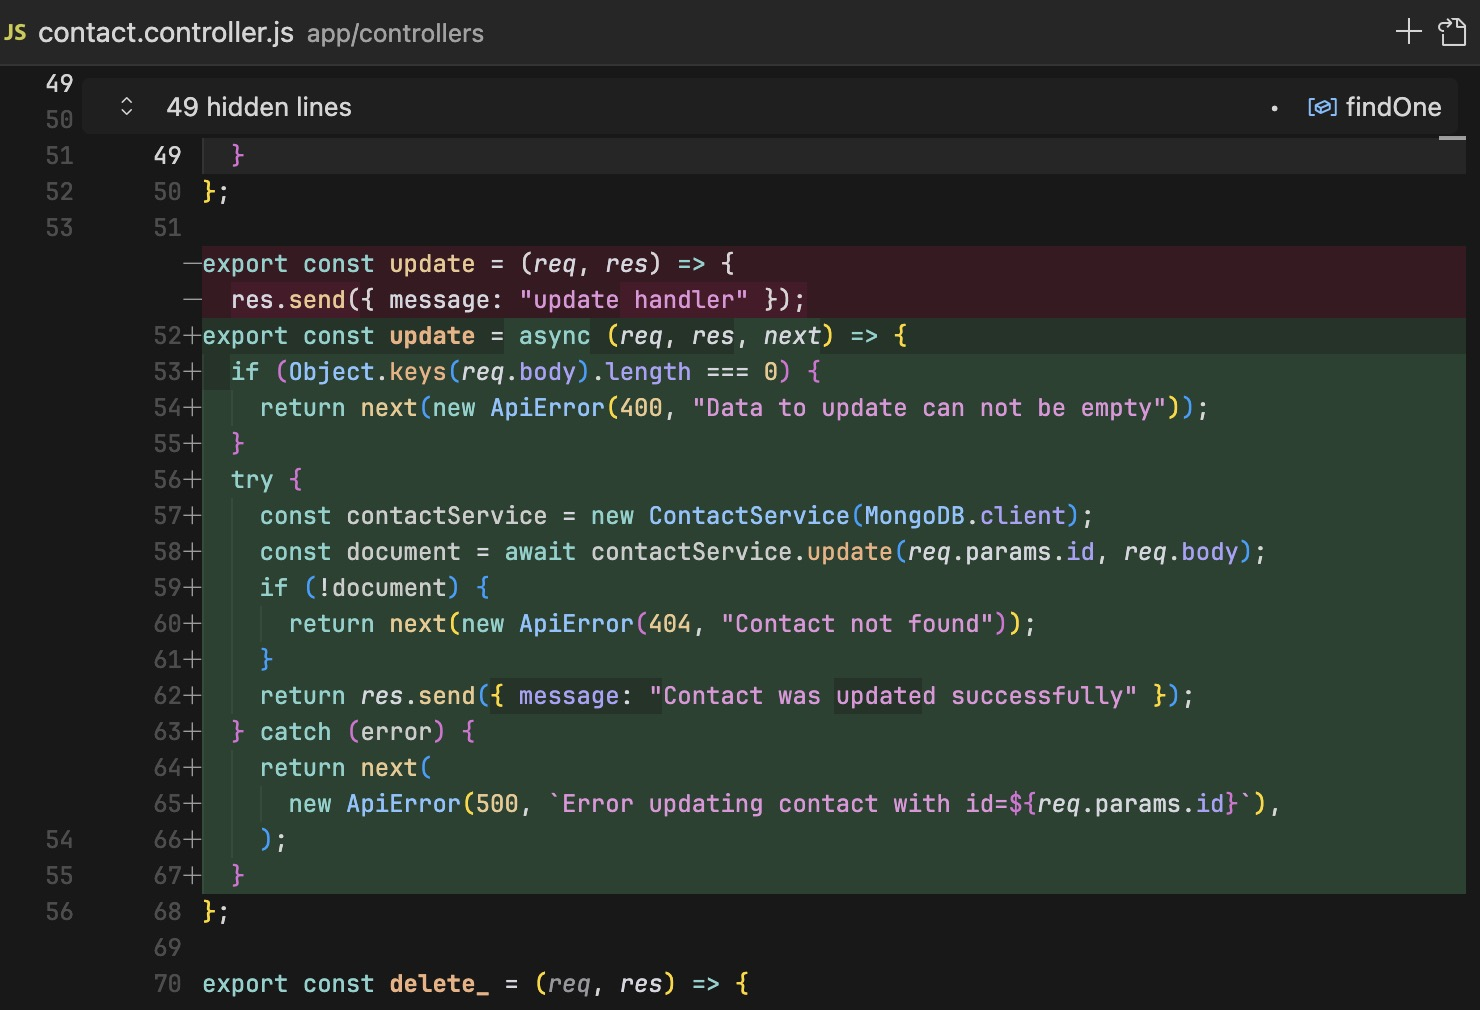
\includegraphics[width=0.8\textwidth]{./assets/handler_update.jpg}
  \caption{Cài đặt handler update}
  \label{fig:contactcontrollerupdate}
\end{figure}

contactService.update(id, document) tìm kiếm tài liệu theo Id và cập nhật tài liệu này với dữ liệu trong đối
tượng document. Phương thức update(id, document) có thế được định nghĩa như sau trong tập tin
app/services/contact.service.js.

\begin{figure}[H]
  \centering
  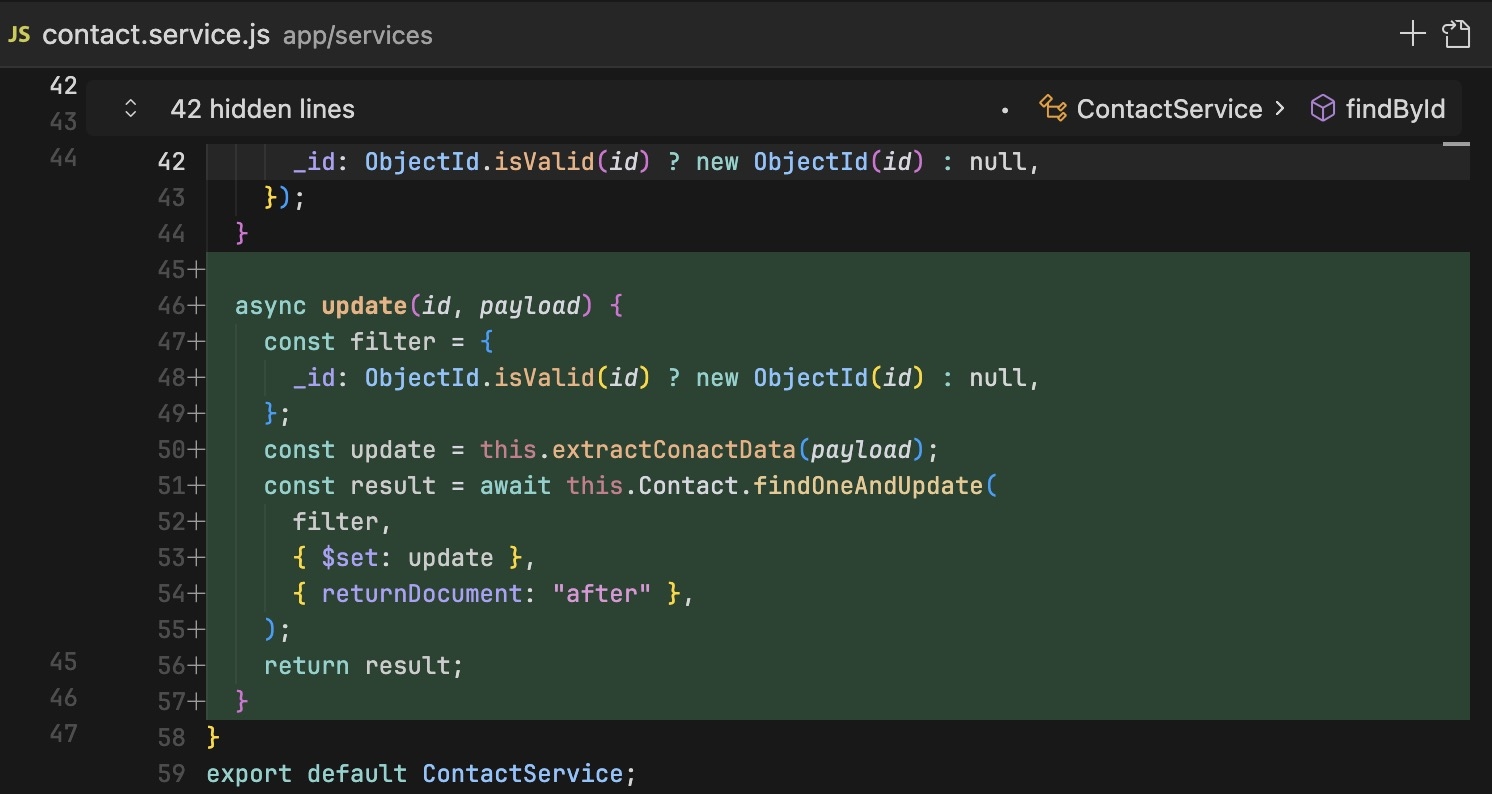
\includegraphics[width=0.8\textwidth]{./assets/update.jpg}
  \caption{Cài đặt hàm update}
  \label{fig:update_function}
\end{figure}

Dùng Postman kiểm tra handler update hoạt động đúng.

\begin{figure}[H]
  \centering
  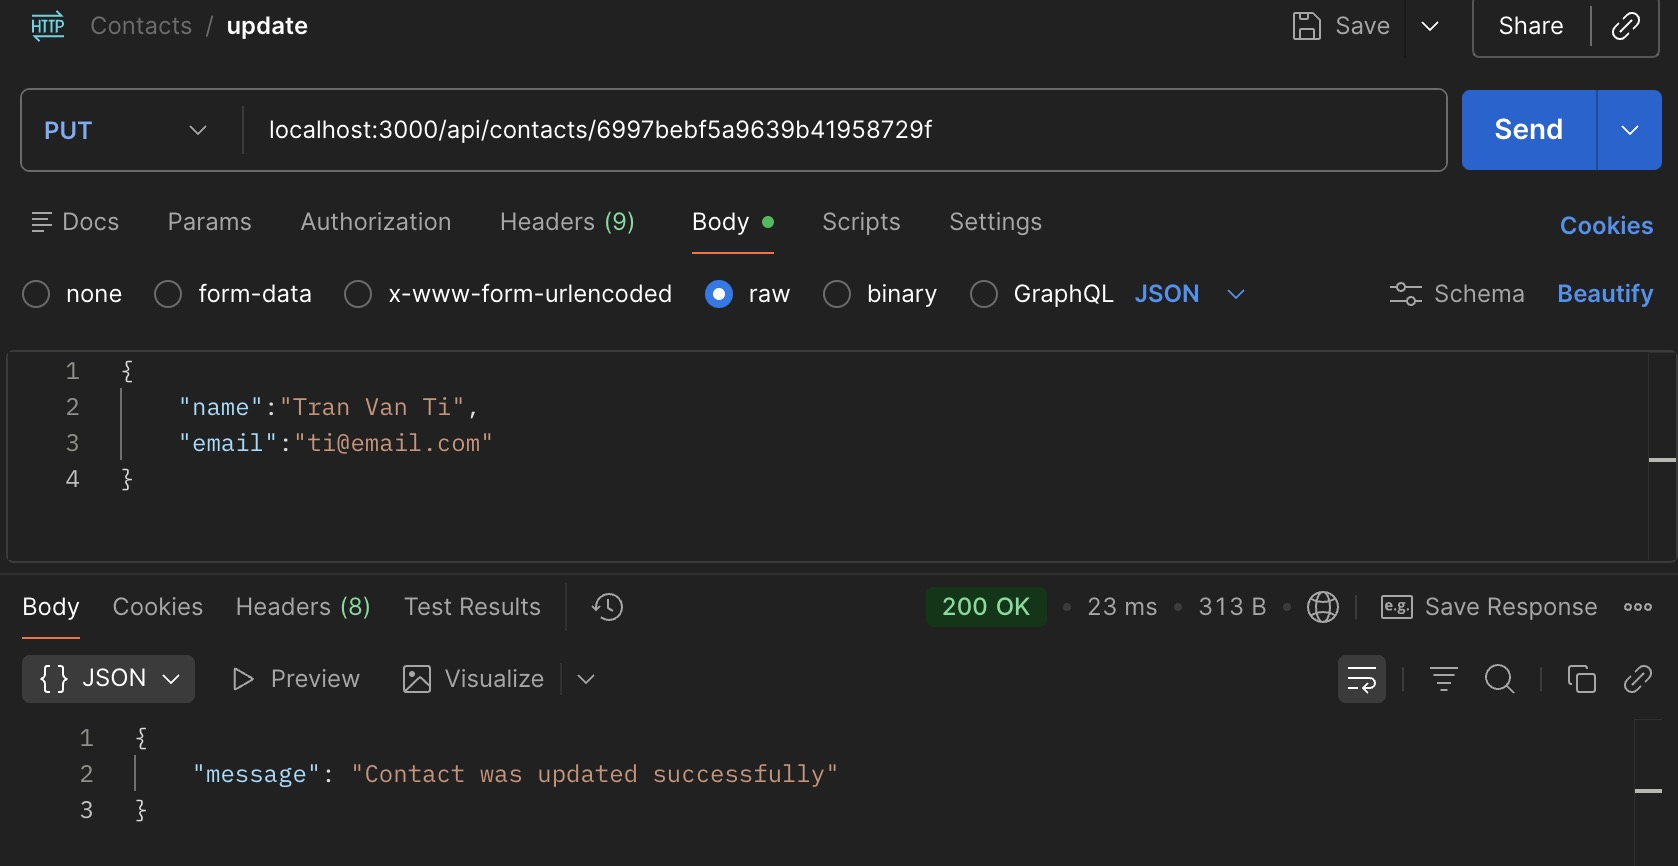
\includegraphics[width=0.8\textwidth]{./assets/postman_update.jpg}
  \caption{Postman update}
  \label{fig:postman_update}
\end{figure}

Kiểm tra data được cập nhật vào MongoDB
\begin{figure}[H]
  \centering
  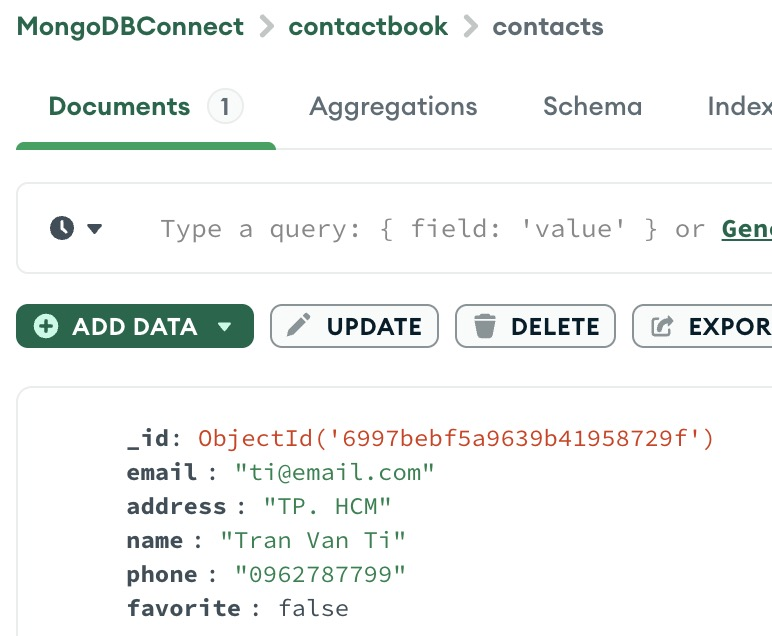
\includegraphics[width=0.8\textwidth]{./assets/mongodb_update.jpg}
  \caption{MongoDB Compass}
  \label{fig:mongodb_update}
\end{figure}

\section{Cài đặt handler delete/deleteAll }

\begin{figure}[H]
  \centering
  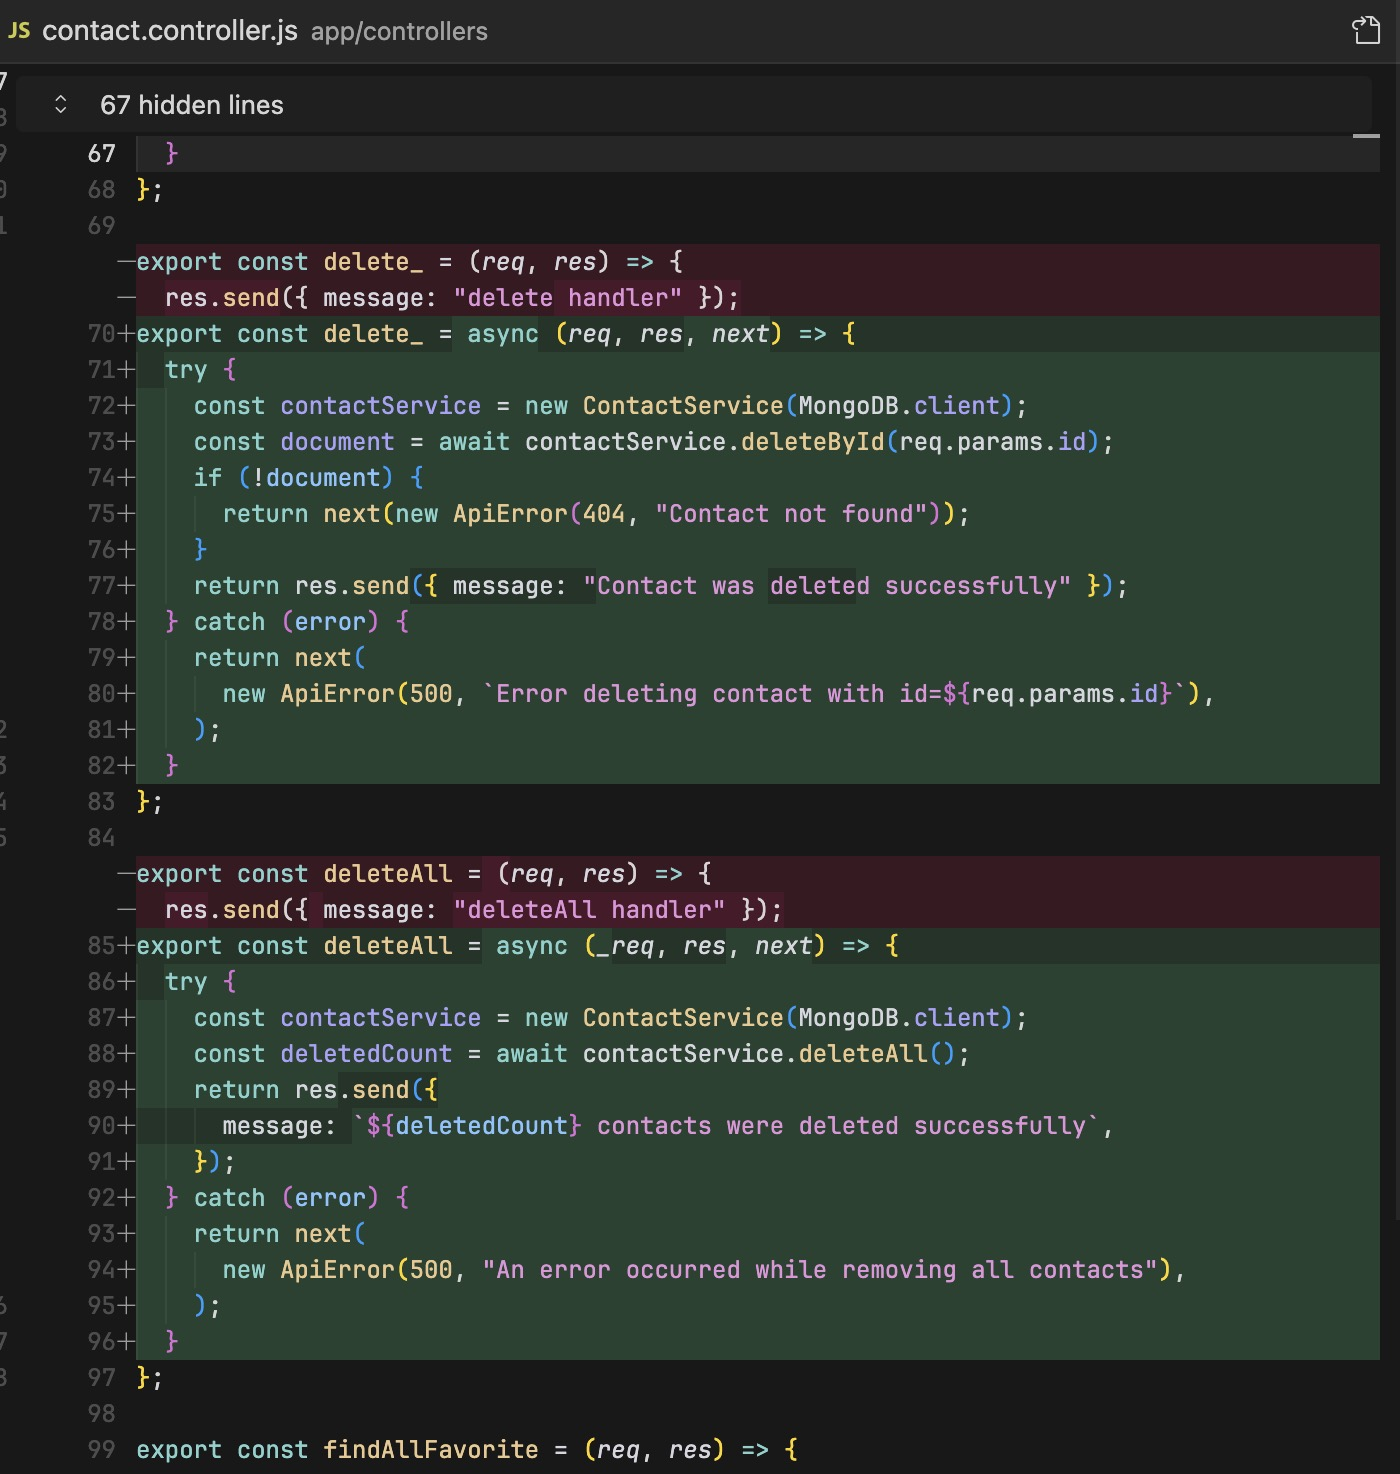
\includegraphics[width=0.8\textwidth]{./assets/handler_delete_deleteAll.jpg}
  \caption{Cài đặt handler delete và handler deleteAll}
  \label{fig:contactcontrollerdelete_deleteAll}
\end{figure}

Cài đặt hàm deleteById và deleteAll 

\begin{figure}[H]
  \centering
  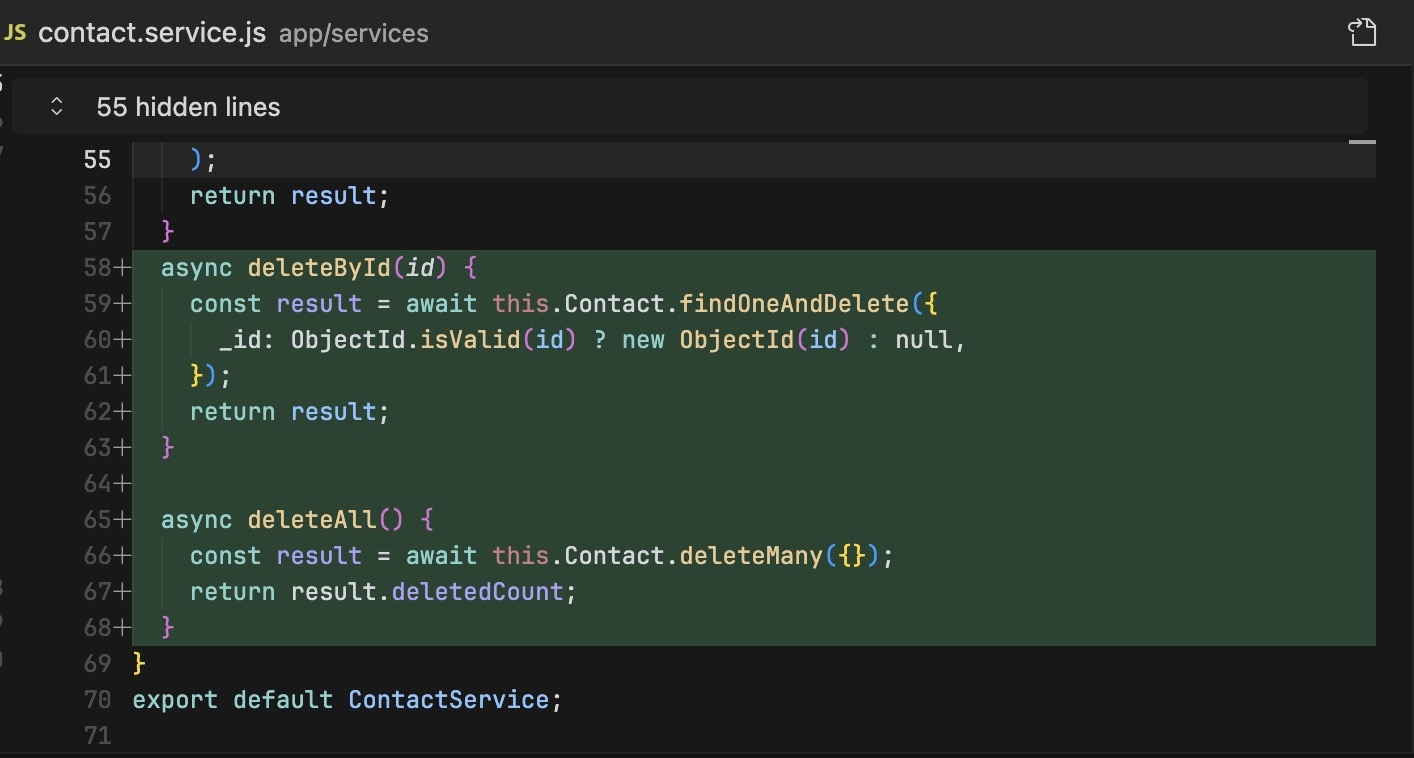
\includegraphics[width=0.8\textwidth]{./assets/deleteById_deleteAll.jpg}
  \caption{Cài đặt hàm deleteById và deleteAll}
  \label{fig:deletebyid_deleteall}
\end{figure}

Dùng Postman kiểm tra handler delete và handler deleteAll hoạt động đúng.

\begin{figure}[H]
  \centering
  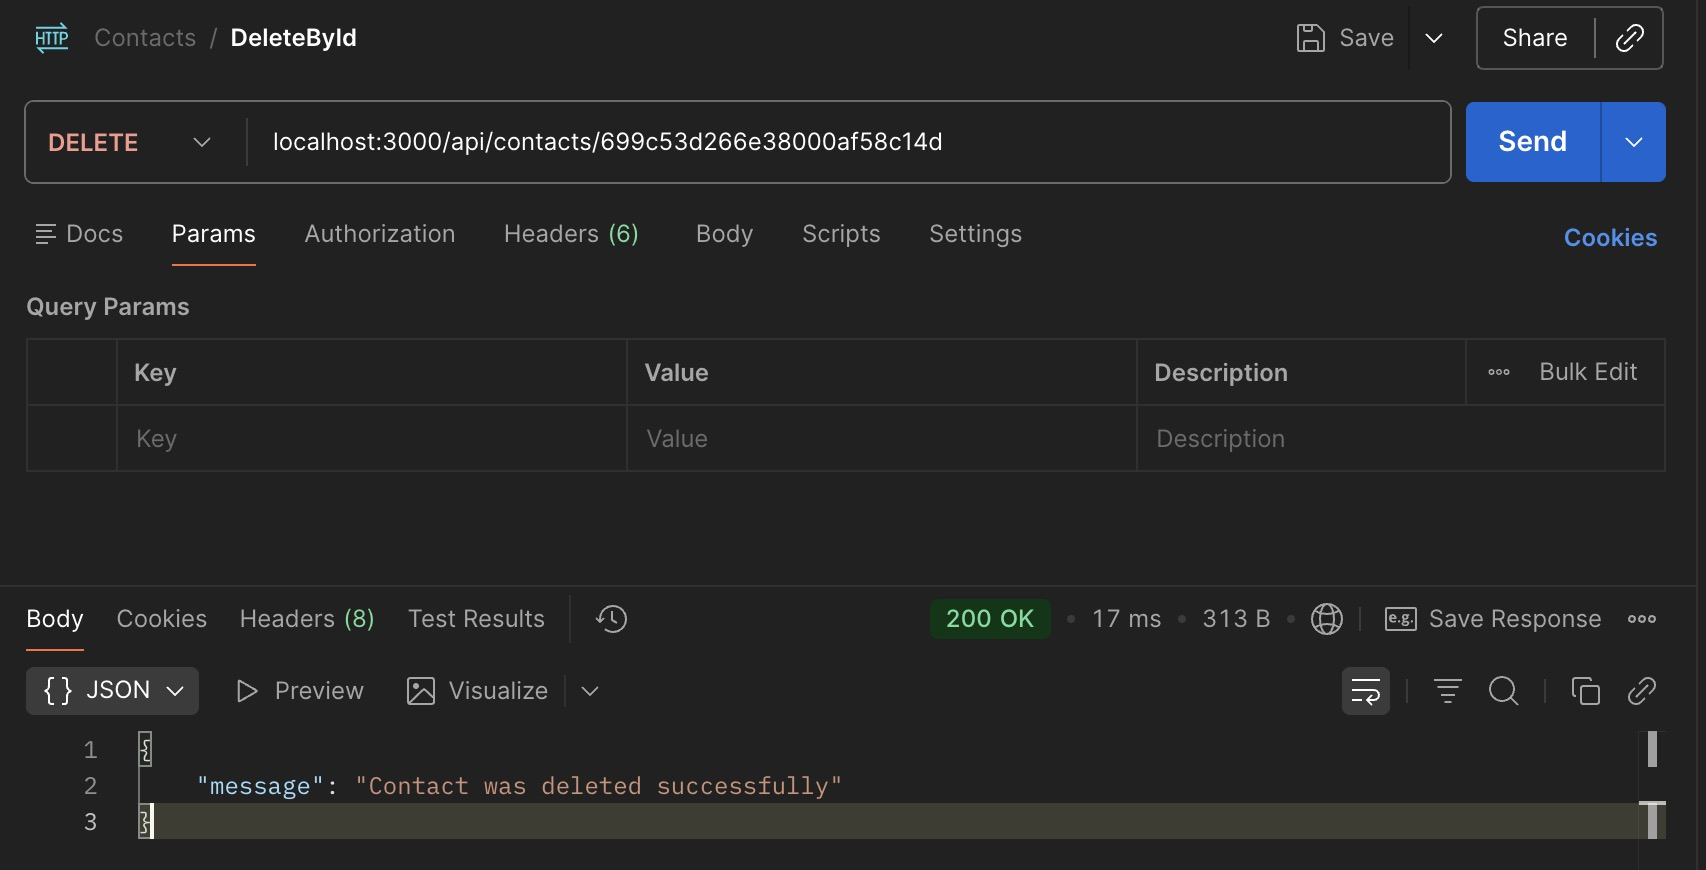
\includegraphics[width=0.8\textwidth]{./assets/postman_delete.jpg}
  \caption{Postman delete}
  \label{fig:postman_delete}
\end{figure}

\begin{figure}[H]
  \centering
  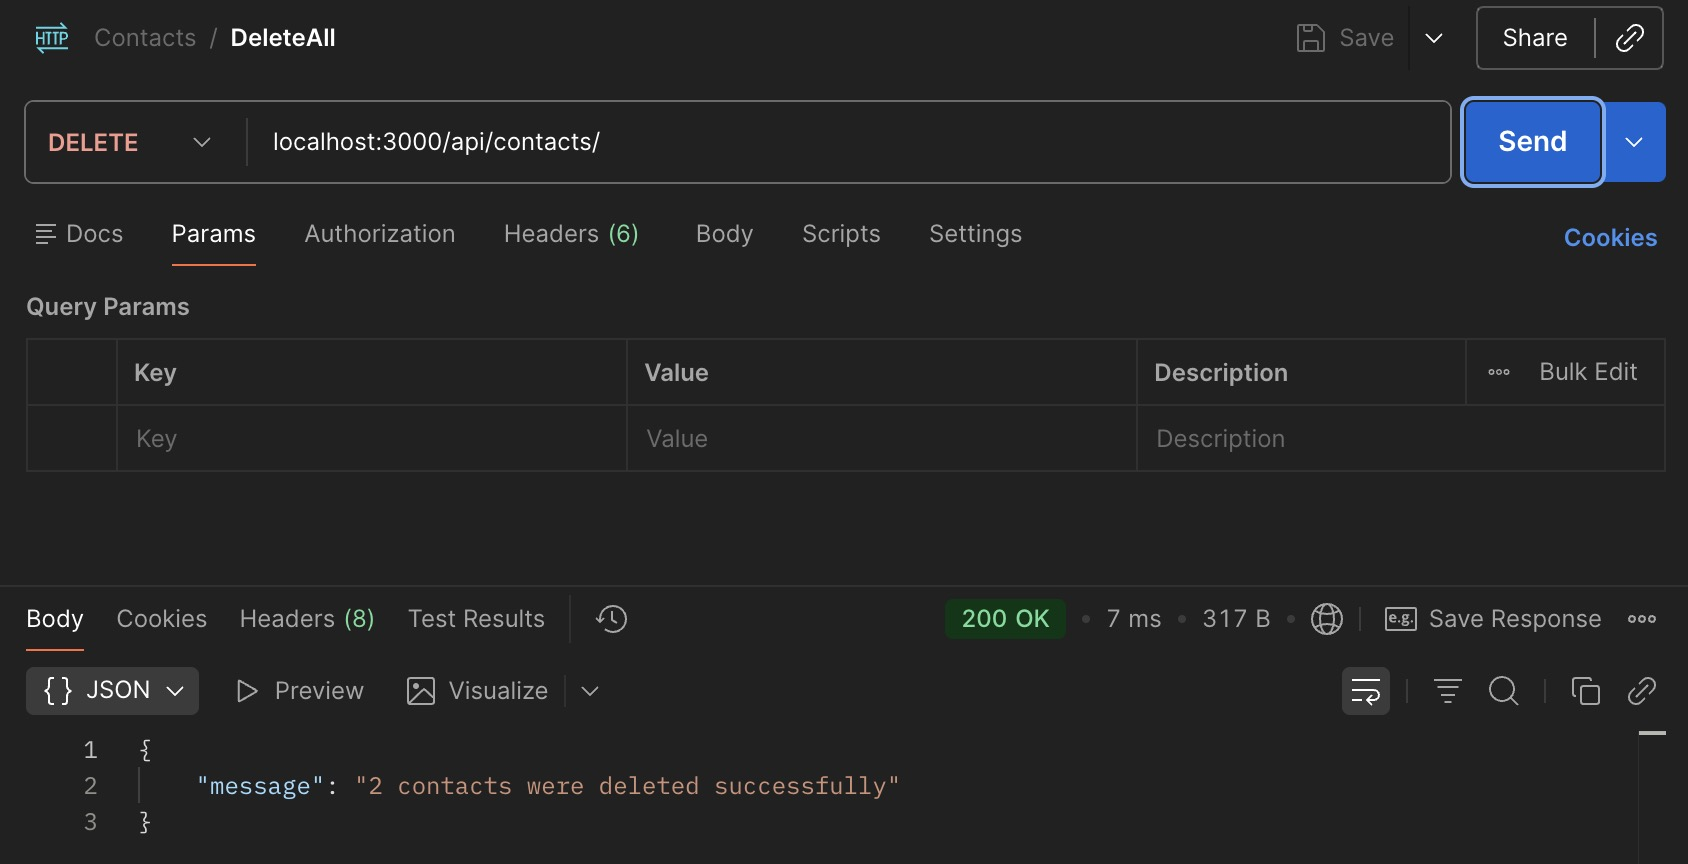
\includegraphics[width=0.8\textwidth]{./assets/postman_deleteAll.jpg}
  \caption{Postman deleteAll}
  \label{fig:postman_deleteAll}
\end{figure}

\section{Phần mở rộng: Login}

Cài đặt route \texttt{auth.route.js} trong thư mục \texttt{app/routes}.

\begin{figure}[H]
  \centering
  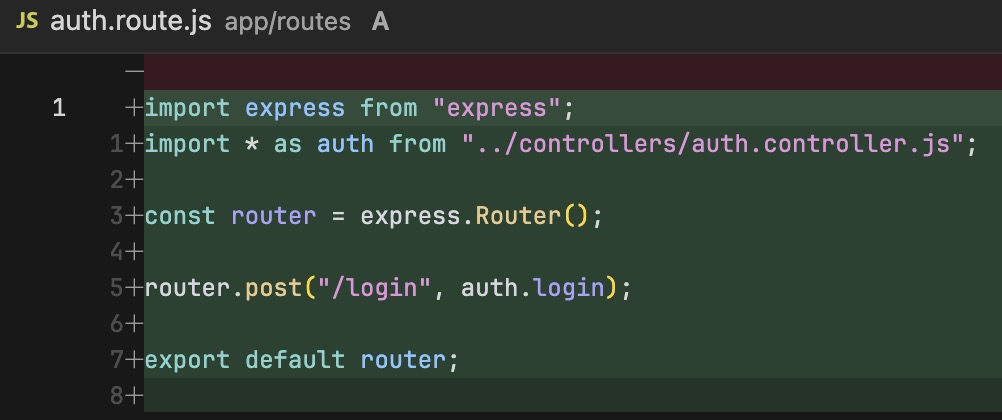
\includegraphics[width=0.8\textwidth]{./assets/auth_route.jpg}
  \caption{Route auth.route.js}
  \label{fig:auth_route}
\end{figure}

Đăng ký route \texttt{auth.route.js} trong file \texttt{app.js}.

\begin{figure}[H]
  \centering
  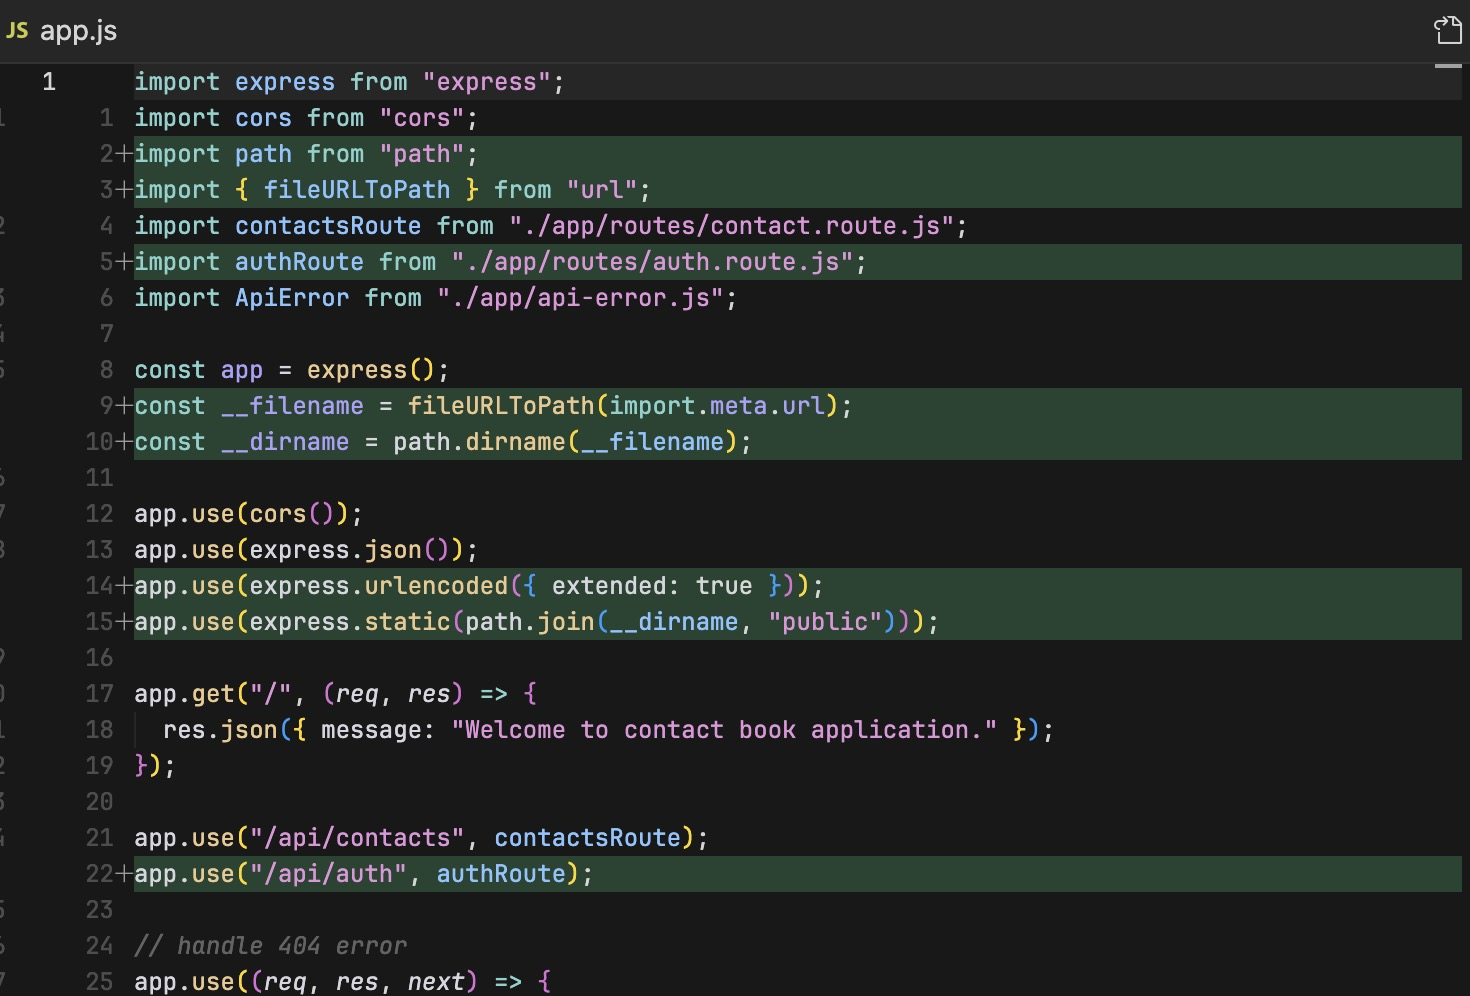
\includegraphics[width=0.8\textwidth]{./assets/app_auth.jpg}
  \caption{Đăng ký route auth.route.js}
  \label{fig:app_auth}
\end{figure}

Tạo form \texttt{login.html} trong thư mục \texttt{public}.

\begin{figure}[H]
  \centering
  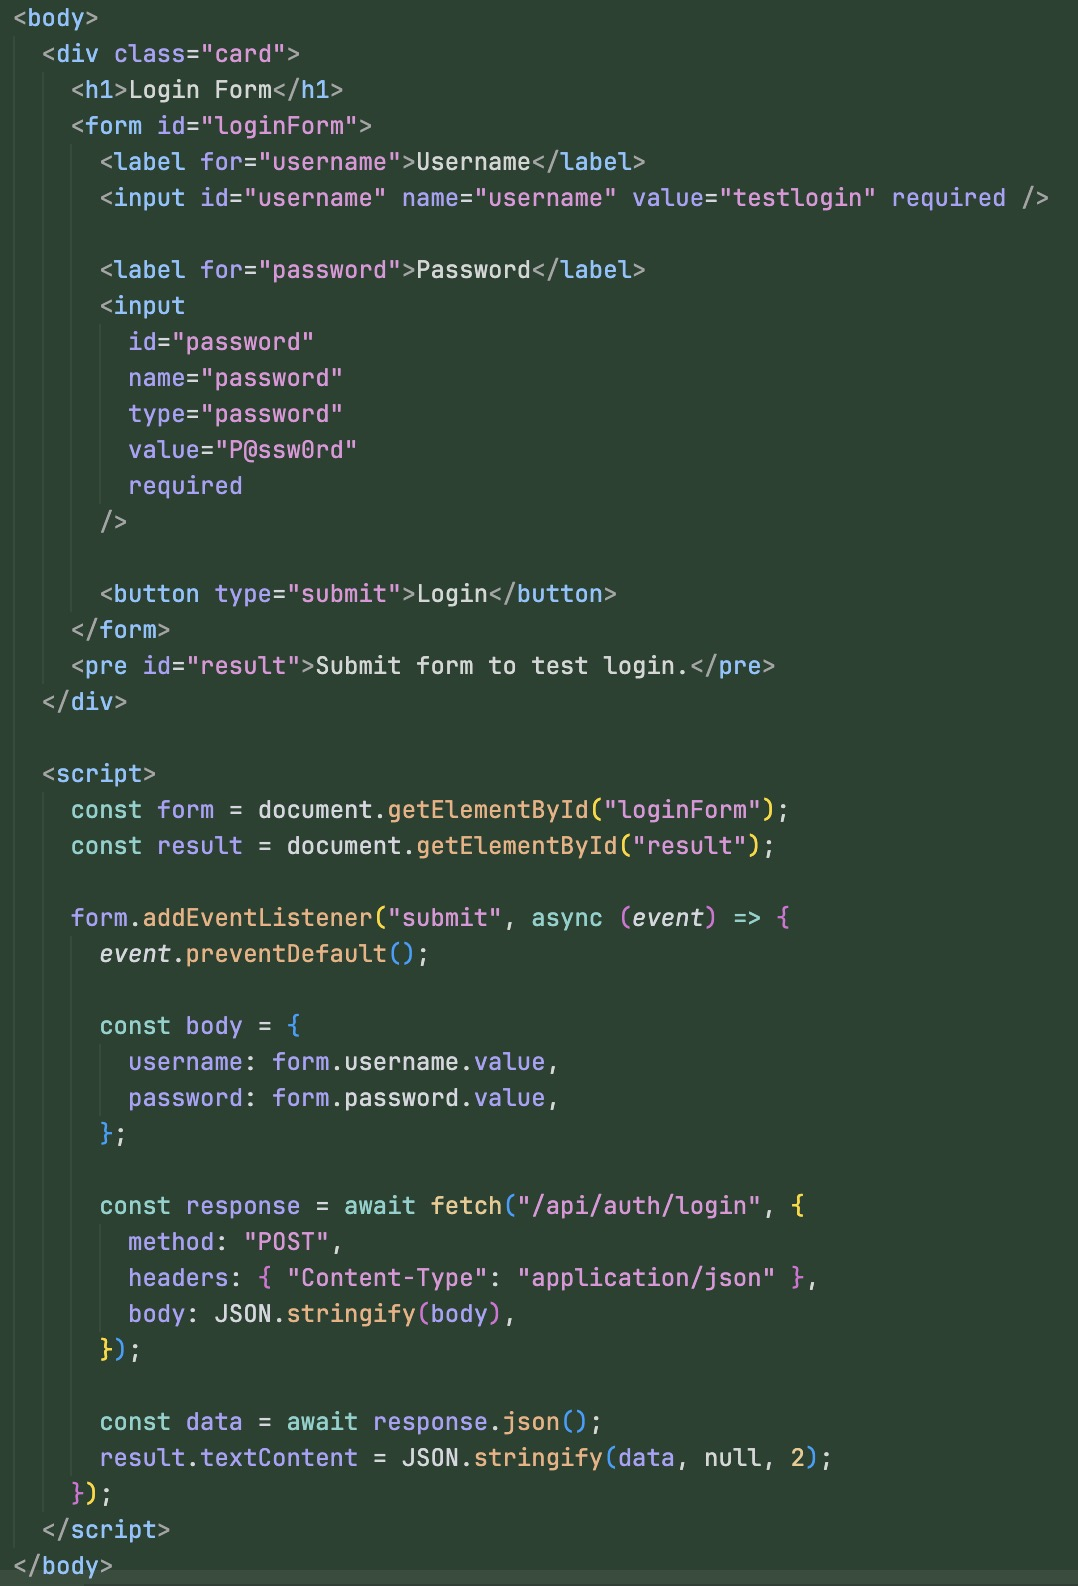
\includegraphics[width=0.6\textwidth]{./assets/login_html.jpg}
  \caption{Form login.html}
  \label{fig:login_form}
\end{figure}

Kiểm tra hoạt động của form login bằng Postman.

\begin{figure}[H]
  \centering
  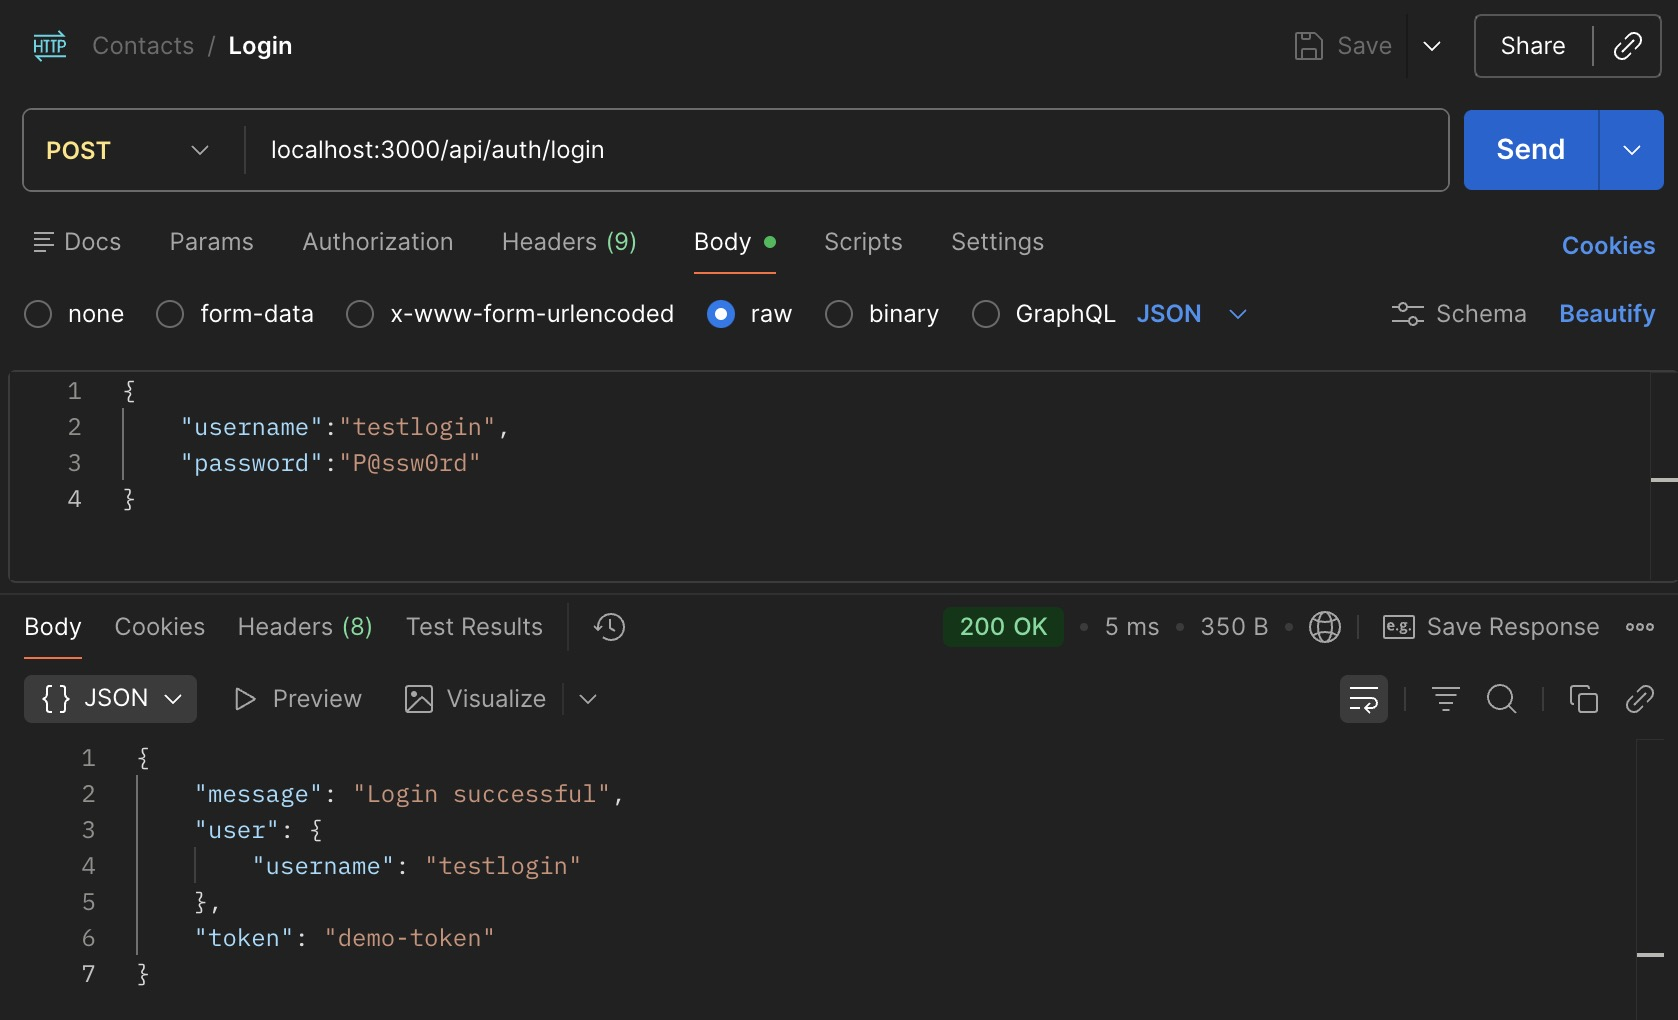
\includegraphics[width=0.8\textwidth]{./assets/postman_test_login.jpg}
  \caption{Postman login}
  \label{fig:postman_login}
\end{figure}

Kiểm tra form login.html hoạt động đúng.

\begin{figure}[H]
  \centering
  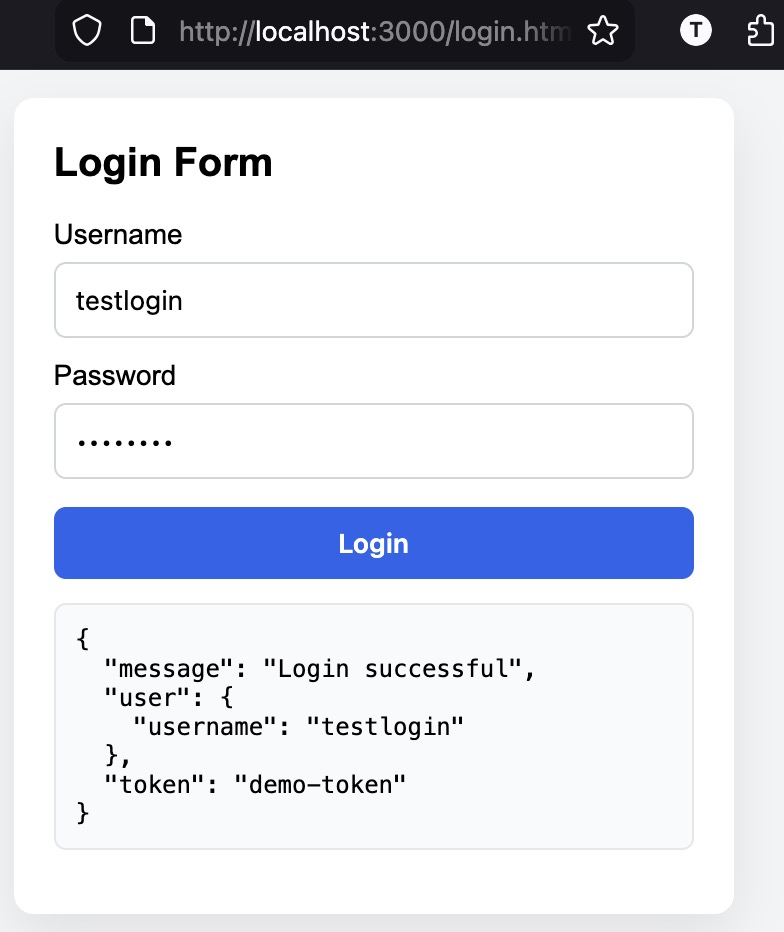
\includegraphics[width=0.6\textwidth]{./assets/login_html_test.jpg}
  \caption{Form login.html hoạt động đúng}
  \label{fig:login_html_test}
\end{figure}

\section{Cấu trúc thư mục dự án BACKEND}

\begin{figure}[H]
  \centering
  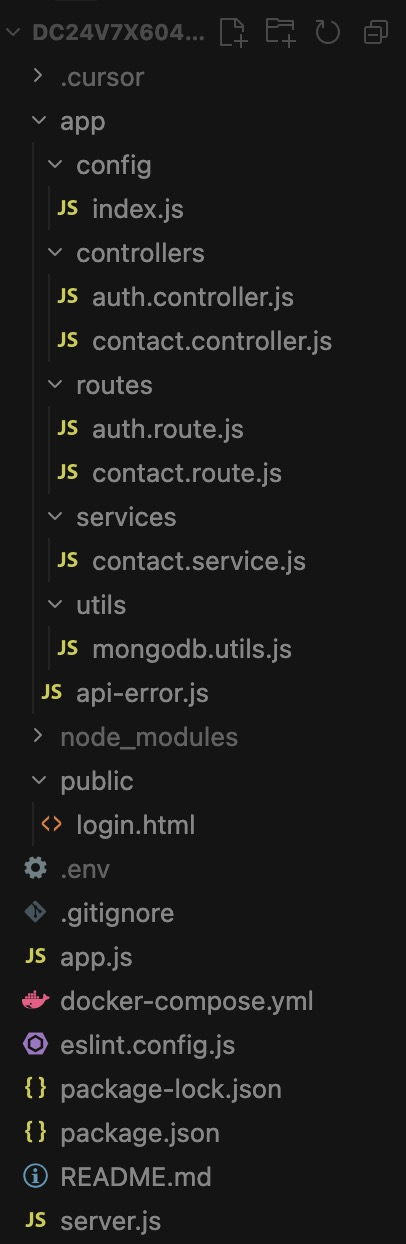
\includegraphics[width=0.4\textwidth]{./assets/project_structure_2.jpg}
  \caption{Cấu trúc thư mục dự án BACKEND}
  \label{fig:project_structure_backend}
\end{figure}


\section{Link Github}

\url{https://github.com/duytechie/DC24V7X604_TranThanhDuy_BACKEND_2}

\end{document}